% Options for packages loaded elsewhere
% Options for packages loaded elsewhere
\PassOptionsToPackage{unicode}{hyperref}
\PassOptionsToPackage{hyphens}{url}
%
\documentclass[
  ignorenonframetext,
  aspectratio=169,
]{beamer}
\newif\ifbibliography
\usepackage{pgfpages}
\setbeamertemplate{caption}[numbered]
\setbeamertemplate{caption label separator}{: }
\setbeamercolor{caption name}{fg=normal text.fg}
\beamertemplatenavigationsymbolsempty
% remove section numbering
\setbeamertemplate{part page}{
  \centering
  \begin{beamercolorbox}[sep=16pt,center]{part title}
    \usebeamerfont{part title}\insertpart\par
  \end{beamercolorbox}
}
\setbeamertemplate{section page}{
  \centering
  \begin{beamercolorbox}[sep=12pt,center]{section title}
    \usebeamerfont{section title}\insertsection\par
  \end{beamercolorbox}
}
\setbeamertemplate{subsection page}{
  \centering
  \begin{beamercolorbox}[sep=8pt,center]{subsection title}
    \usebeamerfont{subsection title}\insertsubsection\par
  \end{beamercolorbox}
}
% Prevent slide breaks in the middle of a paragraph
\widowpenalties 1 10000
\raggedbottom
\AtBeginPart{
  \frame{\partpage}
}
\AtBeginSection{
  \ifbibliography
  \else
    \frame{\sectionpage}
  \fi
}
\AtBeginSubsection{
  \frame{\subsectionpage}
}
\usepackage{iftex}
\ifPDFTeX
  \usepackage[T1]{fontenc}
  \usepackage[utf8]{inputenc}
  \usepackage{textcomp} % provide euro and other symbols
\else % if luatex or xetex
  \usepackage{unicode-math} % this also loads fontspec
  \defaultfontfeatures{Scale=MatchLowercase}
  \defaultfontfeatures[\rmfamily]{Ligatures=TeX,Scale=1}
\fi
\usepackage{lmodern}

\ifPDFTeX\else
  % xetex/luatex font selection
\fi
% Use upquote if available, for straight quotes in verbatim environments
\IfFileExists{upquote.sty}{\usepackage{upquote}}{}
\IfFileExists{microtype.sty}{% use microtype if available
  \usepackage[]{microtype}
  \UseMicrotypeSet[protrusion]{basicmath} % disable protrusion for tt fonts
}{}
\makeatletter
\@ifundefined{KOMAClassName}{% if non-KOMA class
  \IfFileExists{parskip.sty}{%
    \usepackage{parskip}
  }{% else
    \setlength{\parindent}{0pt}
    \setlength{\parskip}{6pt plus 2pt minus 1pt}}
}{% if KOMA class
  \KOMAoptions{parskip=half}}
\makeatother


\usepackage{longtable,booktabs,array}
\usepackage{calc} % for calculating minipage widths
\usepackage{caption}
% Make caption package work with longtable
\makeatletter
\def\fnum@table{\tablename~\thetable}
\makeatother
\usepackage{graphicx}
\makeatletter
\newsavebox\pandoc@box
\newcommand*\pandocbounded[1]{% scales image to fit in text height/width
  \sbox\pandoc@box{#1}%
  \Gscale@div\@tempa{\textheight}{\dimexpr\ht\pandoc@box+\dp\pandoc@box\relax}%
  \Gscale@div\@tempb{\linewidth}{\wd\pandoc@box}%
  \ifdim\@tempb\p@<\@tempa\p@\let\@tempa\@tempb\fi% select the smaller of both
  \ifdim\@tempa\p@<\p@\scalebox{\@tempa}{\usebox\pandoc@box}%
  \else\usebox{\pandoc@box}%
  \fi%
}
% Set default figure placement to htbp
\def\fps@figure{htbp}
\makeatother





\setlength{\emergencystretch}{3em} % prevent overfull lines

\providecommand{\tightlist}{%
  \setlength{\itemsep}{0pt}\setlength{\parskip}{0pt}}



 


\makeatletter
\@ifpackageloaded{caption}{}{\usepackage{caption}}
\AtBeginDocument{%
\ifdefined\contentsname
  \renewcommand*\contentsname{Table of contents}
\else
  \newcommand\contentsname{Table of contents}
\fi
\ifdefined\listfigurename
  \renewcommand*\listfigurename{List of Figures}
\else
  \newcommand\listfigurename{List of Figures}
\fi
\ifdefined\listtablename
  \renewcommand*\listtablename{List of Tables}
\else
  \newcommand\listtablename{List of Tables}
\fi
\ifdefined\figurename
  \renewcommand*\figurename{Figure}
\else
  \newcommand\figurename{Figure}
\fi
\ifdefined\tablename
  \renewcommand*\tablename{Table}
\else
  \newcommand\tablename{Table}
\fi
}
\@ifpackageloaded{float}{}{\usepackage{float}}
\floatstyle{ruled}
\@ifundefined{c@chapter}{\newfloat{codelisting}{h}{lop}}{\newfloat{codelisting}{h}{lop}[chapter]}
\floatname{codelisting}{Listing}
\newcommand*\listoflistings{\listof{codelisting}{List of Listings}}
\makeatother
\makeatletter
\makeatother
\makeatletter
\@ifpackageloaded{caption}{}{\usepackage{caption}}
\@ifpackageloaded{subcaption}{}{\usepackage{subcaption}}
\makeatother

\usepackage{bookmark}
\IfFileExists{xurl.sty}{\usepackage{xurl}}{} % add URL line breaks if available
\urlstyle{same}
\hypersetup{
  pdftitle={Análise de Agrupamentos},
  hidelinks,
  pdfcreator={LaTeX via pandoc}}



\title{Análise de Agrupamentos}
\author{}
\date{}

\begin{document}
\frame{\titlepage}


\begin{frame}{O que é clustering?}
\phantomsection\label{o-que-uxe9-clustering}
É uma \textbf{técnica estatística multivariada} para identificar
agrupamentos dos dados de acordo com o grau de semelhança. Queremos
achar um grupo de objetos, que são similares entre si e diferentes de
outros grupos.

\begin{figure}

\begin{minipage}{0.50\linewidth}
\begin{center}
\pandocbounded{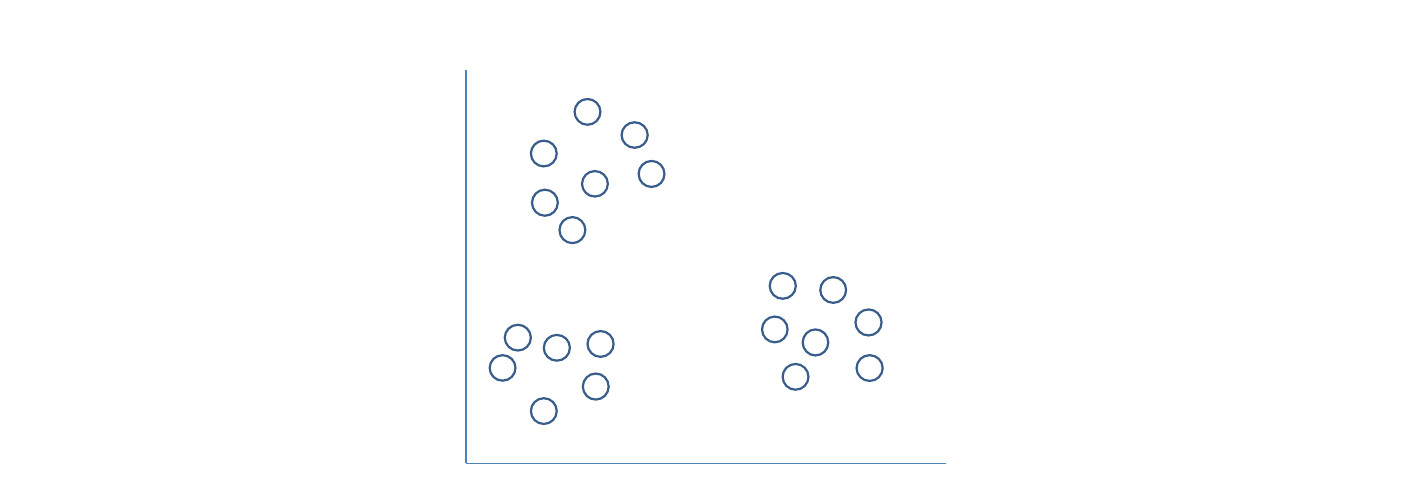
\includegraphics[keepaspectratio]{../../images/AA/grafico_AA-01.jpg}}
\end{center}
\end{minipage}%
%
\begin{minipage}{0.50\linewidth}
\begin{center}
\pandocbounded{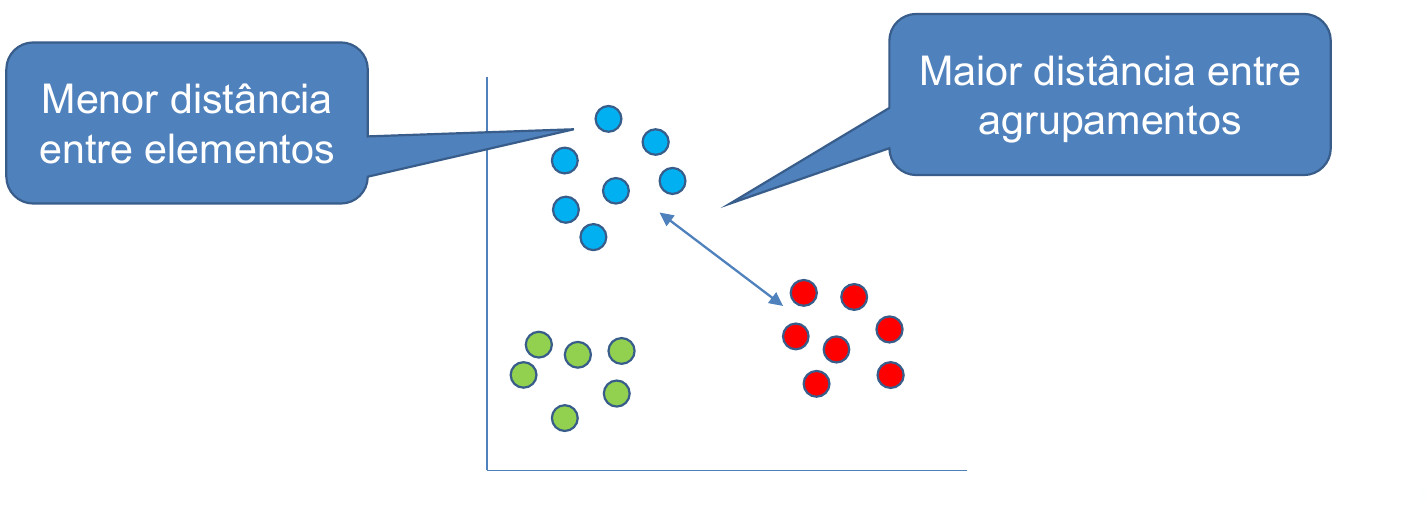
\includegraphics[keepaspectratio]{../../images/AA/grafico_AA-02.jpg}}
\end{center}
\end{minipage}%

\end{figure}%

\begin{itemize}
\tightlist
\item
  O \textbf{objetivo} típico em clustering é descobrir os ``agrupamentos
  naturais'' presente nos dados.
\end{itemize}
\end{frame}

\begin{frame}{O que é clustering?}
\phantomsection\label{o-que-uxe9-clustering-1}
\begin{itemize}
\tightlist
\item
  Conjunto de dados \textbf{contendo} agrupamentos ``naturais'':
\end{itemize}

\begin{center}
\pandocbounded{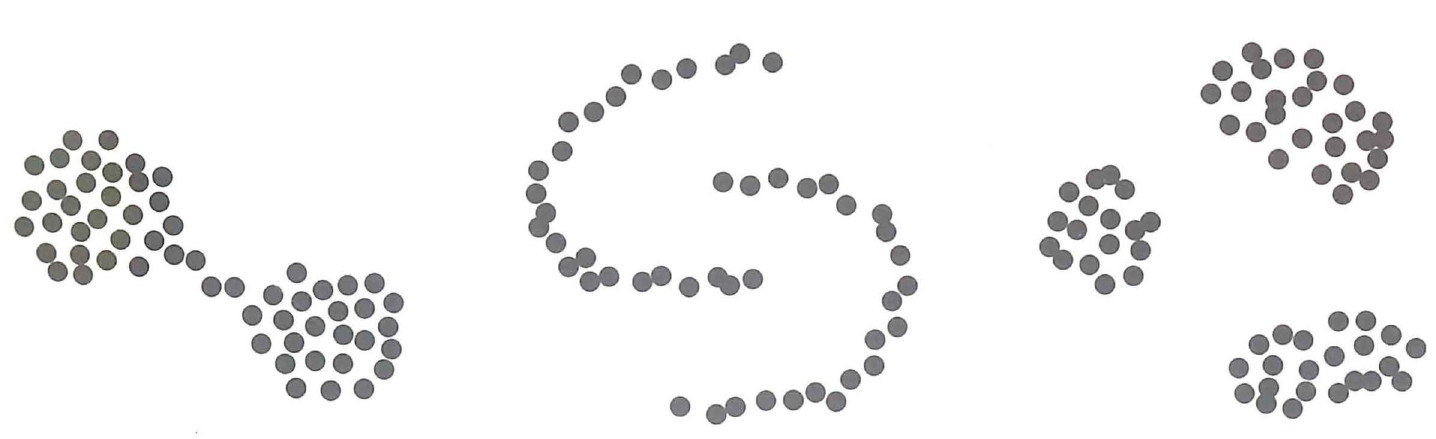
\includegraphics[keepaspectratio]{../../images/AA/grupos_naturais.jpg}}
\end{center}
\end{frame}

\begin{frame}{O que é clustering?}
\phantomsection\label{o-que-uxe9-clustering-2}
\begin{itemize}
\tightlist
\item
  Conjunto de dados \textbf{sem} agrupamentos ``naturais'':
\end{itemize}

\begin{center}
\pandocbounded{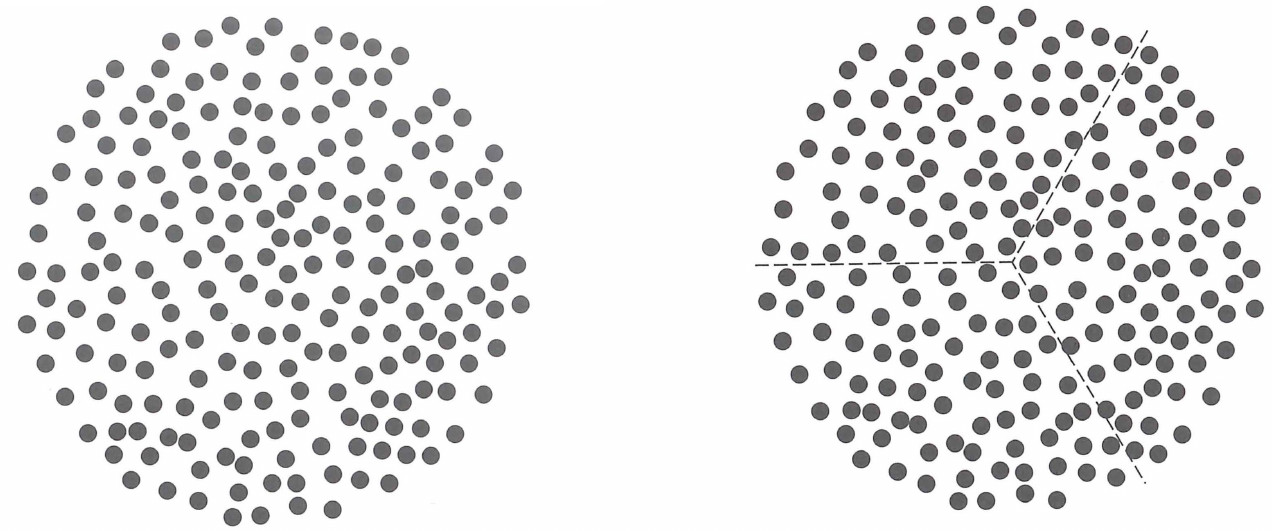
\includegraphics[keepaspectratio]{../../images/AA/grupos_nao_naturais.jpg}}
\end{center}
\end{frame}

\begin{frame}{Tendência de agrupamentos: ``Faz sentido aplicar um
algoritmo de clusterização nesses dados?''}
\phantomsection\label{tenduxeancia-de-agrupamentos-faz-sentido-aplicar-um-algoritmo-de-clusterizauxe7uxe3o-nesses-dados}
\begin{block}{\textbf{Método estatístico:} Estatística de Hopkins}
\phantomsection\label{muxe9todo-estatuxedstico-estatuxedstica-de-hopkins}
A \textbf{Estatística de Hopkins} é uma medida pré-clusterização muito
usada para avaliar se um conjunto de dados apresenta tendência natural à
formação de agrupamentos (clusters) ou se os pontos estão distribuídos
de forma aproximadamente aleatória no espaço das variáveis.
\end{block}
\end{frame}

\begin{frame}{Tendência de agrupamentos: ``Faz sentido aplicar um
algoritmo de clusterização nesses dados?''}
\phantomsection\label{tenduxeancia-de-agrupamentos-faz-sentido-aplicar-um-algoritmo-de-clusterizauxe7uxe3o-nesses-dados-1}
\begin{block}{\textbf{Método estatístico:} Estatística de Hopkins}
\phantomsection\label{muxe9todo-estatuxedstico-estatuxedstica-de-hopkins-1}
\begin{itemize}
\tightlist
\item
  A ideia central é comparar distâncias:

  \begin{itemize}
  \tightlist
  \item
    Distâncias entre pontos reais do conjunto de dados
  \item
    Distâncias entre pontos artificiais gerados aleatoriamente no mesmo
    espaço amostral
  \end{itemize}
\item
  Se os dados tiverem estrutura de clusters, os pontos reais tendem a
  estar mais próximos entre si do que pontos gerados aleatoriamente.
\end{itemize}
\end{block}
\end{frame}

\begin{frame}{Tendência de agrupamentos: ``Faz sentido aplicar um
algoritmo de clusterização nesses dados?''}
\phantomsection\label{tenduxeancia-de-agrupamentos-faz-sentido-aplicar-um-algoritmo-de-clusterizauxe7uxe3o-nesses-dados-2}
\begin{block}{\textbf{Método estatístico:} Estatística de Hopkins}
\phantomsection\label{muxe9todo-estatuxedstico-estatuxedstica-de-hopkins-2}
\begin{itemize}
\tightlist
\item
  Considerando um inteiro \(m \ll n\), de pontos amostrados
  (normalizados), calcula-se a distância de cada ponto até o vizinho
  mais próximo, excluindo o próprio ponto
\end{itemize}

\[
w_i
=
\min_{x_j \in X \setminus \{x_i\}}
d(x_i, x_j),
\qquad i = 1,\ldots,m
\]
\end{block}
\end{frame}

\begin{frame}{Tendência de agrupamentos: ``Faz sentido aplicar um
algoritmo de clusterização nesses dados?''}
\phantomsection\label{tenduxeancia-de-agrupamentos-faz-sentido-aplicar-um-algoritmo-de-clusterizauxe7uxe3o-nesses-dados-3}
\begin{block}{\textbf{Método estatístico:} Estatística de Hopkins}
\phantomsection\label{muxe9todo-estatuxedstico-estatuxedstica-de-hopkins-3}
\begin{itemize}
\tightlist
\item
  Geram-se \(m\) pontos artificiais \(y_1, \ldots, y_m\), assumindo
  distribuição uniforme no hipercubo definido pelos limites dos dados e
  independência entre as dimensões. Para cada ponto artificial \(j\),
  calcula-se a distância até o vizinho mais próximo no conjunto real.
\end{itemize}

\[
u_i
=
\min_{x \in X}
d(y_i, x),
\qquad i = 1,\ldots,m
\]
\end{block}
\end{frame}

\begin{frame}{Tendência de agrupamentos: ``Faz sentido aplicar um
algoritmo de clusterização nesses dados?''}
\phantomsection\label{tenduxeancia-de-agrupamentos-faz-sentido-aplicar-um-algoritmo-de-clusterizauxe7uxe3o-nesses-dados-4}
\begin{block}{\textbf{Método estatístico:} Estatística de Hopkins}
\phantomsection\label{muxe9todo-estatuxedstico-estatuxedstica-de-hopkins-4}
\[H = \dfrac{\sum \limits_{i=1}^m u_i}{\sum \limits_{i=1}^m u_i + \sum \limits_{i=1}^m w_i}\]

\begin{itemize}
\item
  \(w_i\): distância do ponto real ao vizinho mais próximo
\item
  \(u_i\): distância do ponto artificial ao ponto real mais próximo
\end{itemize}
\end{block}
\end{frame}

\begin{frame}{Tendência de agrupamentos: ``Faz sentido aplicar um
algoritmo de clusterização nesses dados?''}
\phantomsection\label{tenduxeancia-de-agrupamentos-faz-sentido-aplicar-um-algoritmo-de-clusterizauxe7uxe3o-nesses-dados-5}
\begin{block}{Interpretação da Estatística de Hopkins}
\phantomsection\label{interpretauxe7uxe3o-da-estatuxedstica-de-hopkins}
Sob a hipótese de ausência de clusters (padrão de referência), espera-se
que as distâncias \(u_i\) e \(w_i\) sejam, em média, comparáveis, o que
leva a: \[
H \approx 0.5
\]

Em termos práticos:

\begin{itemize}
\tightlist
\item
  \(H \approx 0.5\): dados compatíveis com \textbf{padrão aleatório}
  (baixa tendência à clusterização);
\item
  \(H > 0.5\): evidência de \textbf{tendência à formação de clusters}
  (quanto mais próximo de 1, mais agregado);
\item
  \(H < 0.5\): padrão mais \textbf{regular ou espalhado} do que o
  aleatório.
\end{itemize}
\end{block}
\end{frame}

\begin{frame}{Tendência de agrupamentos: ``Faz sentido aplicar um
algoritmo de clusterização nesses dados?''}
\phantomsection\label{tenduxeancia-de-agrupamentos-faz-sentido-aplicar-um-algoritmo-de-clusterizauxe7uxe3o-nesses-dados-6}
\begin{block}{Interpretação da Estatística de Hopkins}
\phantomsection\label{interpretauxe7uxe3o-da-estatuxedstica-de-hopkins-1}
\begin{quote}
\textbf{Observação:} como \(H\) depende de amostragem aleatória (seleção
dos \(m\) pontos e geração dos pontos artificiais), é recomendável
repetir o cálculo várias vezes e resumir o resultado por média ou
mediana.
\end{quote}
\end{block}
\end{frame}

\begin{frame}{Tendência de agrupamentos}
\phantomsection\label{tenduxeancia-de-agrupamentos}
\begin{block}{\textbf{Método visual:} Avaliação visual da tendência de
agrupamento (VAT)}
\phantomsection\label{muxe9todo-visual-avaliauxe7uxe3o-visual-da-tenduxeancia-de-agrupamento-vat}
\begin{itemize}
\item
  A Avaliação Visual da Tendência de Agrupamento (VAT) é um método
  exploratório que avalia, de forma gráfica, se um conjunto de dados
  apresenta evidência de agrupamentos naturais.
\item
  O procedimento baseia-se na matriz de distâncias entre as observações.
  Após o cálculo da matriz \[
  D = [d(x_i,x_j)]_{n\times n},
  \] as observações são reordenadas de modo que pontos similares fiquem
  próximos, e a matriz resultante é exibida como um mapa de calor.
\end{itemize}
\end{block}
\end{frame}

\begin{frame}{Tendência de agrupamentos}
\phantomsection\label{tenduxeancia-de-agrupamentos-1}
\begin{block}{\textbf{Método visual:} Avaliação visual da tendência de
agrupamento (VAT)}
\phantomsection\label{muxe9todo-visual-avaliauxe7uxe3o-visual-da-tenduxeancia-de-agrupamento-vat-1}
\begin{center}
\pandocbounded{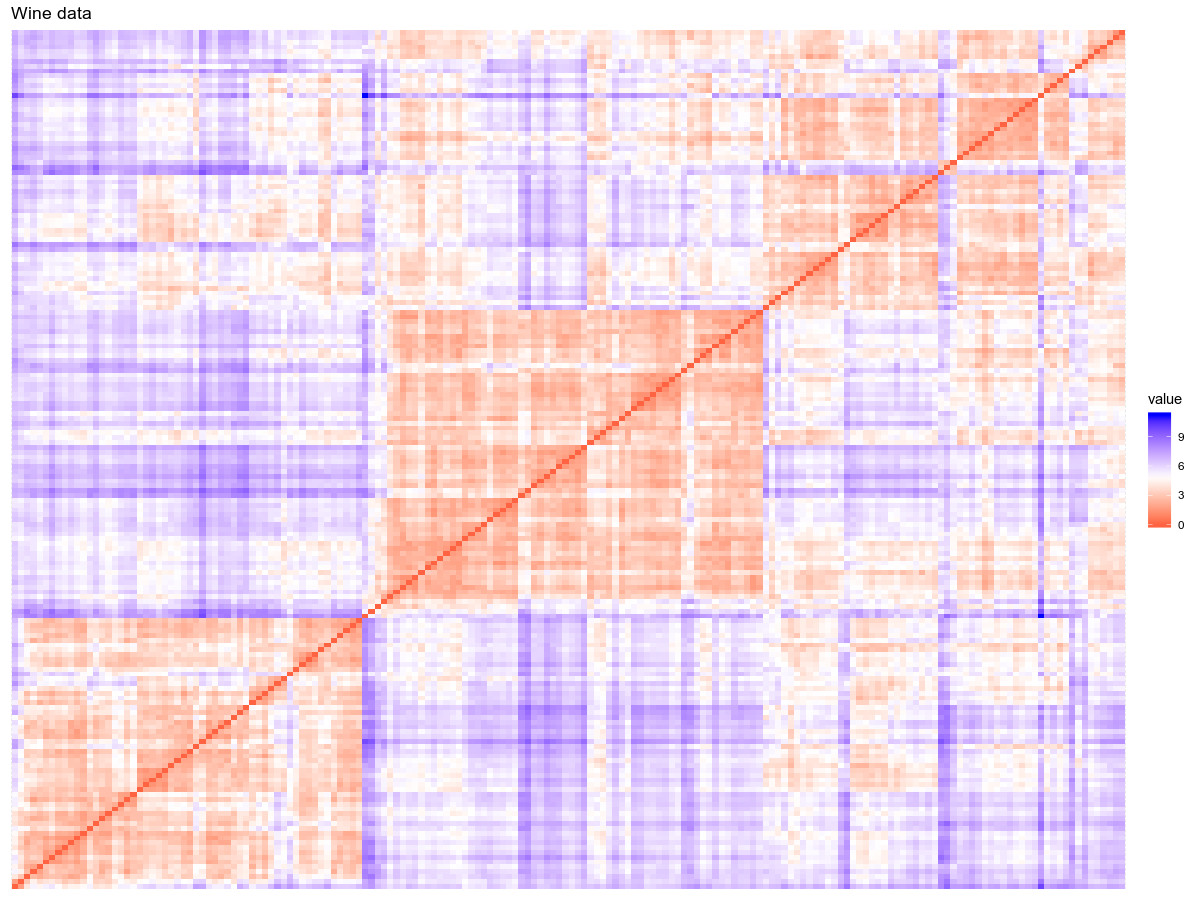
\includegraphics[keepaspectratio]{../../images/AA/metodo_visual.jpg}}
\end{center}
\end{block}
\end{frame}

\begin{frame}{Tendência de agrupamentos}
\phantomsection\label{tenduxeancia-de-agrupamentos-2}
\begin{block}{\textbf{Método visual:} Avaliação visual da tendência de
agrupamento (VAT)}
\phantomsection\label{muxe9todo-visual-avaliauxe7uxe3o-visual-da-tenduxeancia-de-agrupamento-vat-2}
\begin{itemize}
\tightlist
\item
  A interpretação é feita visualmente:

  \begin{itemize}
  \tightlist
  \item
    blocos escuros ao longo da diagonal indicam possível presença de
    clusters;
  \item
    ausência de blocos bem definidos sugere padrão aleatório ou ausência
    de estrutura de agrupamento.
  \end{itemize}
\item
  O VAT é uma ferramenta pré-clusterização e deve ser utilizado de forma
  complementar a medidas quantitativas, como a Estatística de Hopkins.
\end{itemize}
\end{block}
\end{frame}

\begin{frame}{Que perguntas a clusterização pode responder?}
\phantomsection\label{que-perguntas-a-clusterizauxe7uxe3o-pode-responder}
A clusterização é uma técnica de aprendizado não supervisionado cujo
objetivo é identificar grupos de observações semelhantes, sem rótulos
prévios. Ela é usada tanto como \textbf{objetivo final} quanto como
\textbf{ferramenta de apoio à decisão}.

\pause

\begin{itemize}
\tightlist
\item
  \textbf{Como agrupo os clientes que compram no site?}\\
  A clusterização permite identificar perfis de clientes com
  comportamentos de compra semelhantes, apoiando estratégias de
  segmentação e marketing.
\end{itemize}

\pause

\begin{itemize}
\tightlist
\item
  \textbf{Onde coloco uma antena de operadora de celular?}\\
  A partir da clusterização espacial de usuários ou regiões, é possível
  identificar áreas de alta concentração de demanda, sugerindo locais
  estratégicos para instalação.
\end{itemize}
\end{frame}

\begin{frame}{Que perguntas a clusterização pode responder?}
\phantomsection\label{que-perguntas-a-clusterizauxe7uxe3o-pode-responder-1}
\begin{itemize}
\tightlist
\item
  \textbf{Onde deixo uma ambulância estacionada para atender uma
  emergência?}\\
  A clusterização de ocorrências passadas ajuda a identificar zonas
  críticas, auxiliando na alocação eficiente de recursos de emergência.
\end{itemize}

\pause

\begin{itemize}
\tightlist
\item
  \textbf{Como classifico cervejas em categorias distintas?}\\
  A clusterização explora similaridades entre produtos e pode revelar
  categorias naturais ou estilos semelhantes, apoiando a construção de
  classificações.
\end{itemize}
\end{frame}

\begin{frame}{Algumas questões\ldots{}}
\phantomsection\label{algumas-questuxf5es}
🤔 Como medir a homogeneidade entre indivíduos?

🤔 E entre grupos de indivíduos?

🤔 Dado um conjunto de indivíduos, quantos grupos posso formar?
\end{frame}

\begin{frame}{Algumas questões\ldots{}}
\phantomsection\label{algumas-questuxf5es-1}
Imagine que você tenha 16 cartas figuradas (\(A,K,Q,J\)) e que queira
formar grupos de cartas semelhantes\ldots{}

\begin{figure}

\begin{minipage}{0.70\linewidth}
\begin{center}
\pandocbounded{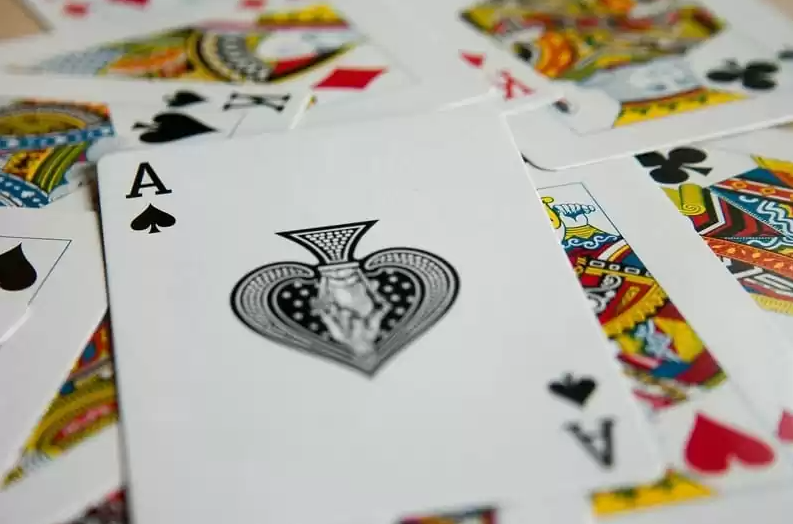
\includegraphics[keepaspectratio]{../../images/AA/bar.png}}
\end{center}
\end{minipage}%
%
\begin{minipage}{0.30\linewidth}
\textbf{Como você formaria esses grupos?}\end{minipage}%

\end{figure}%
\end{frame}

\begin{frame}{Algumas questões\ldots{}}
\phantomsection\label{algumas-questuxf5es-2}
\begin{figure}

\begin{minipage}{0.50\linewidth}

\begin{figure}[H]

{\centering 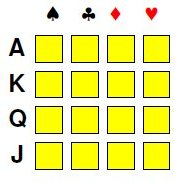
\includegraphics[width=0.85\linewidth,height=\textheight,keepaspectratio]{../../images/AA/barsit1.jpg}

}

\subcaption{Cartas individuais?}

\end{figure}%

\end{minipage}%
%
\begin{minipage}{0.50\linewidth}

\begin{figure}[H]

{\centering 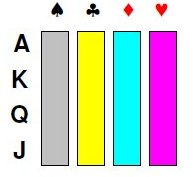
\includegraphics[width=0.9\linewidth,height=\textheight,keepaspectratio]{../../images/AA/barsit2.jpg}

}

\subcaption{Agrupar por naipes?}

\end{figure}%

\end{minipage}%

\end{figure}%
\end{frame}

\begin{frame}{Algumas questões\ldots{}}
\phantomsection\label{algumas-questuxf5es-3}
\begin{figure}

\begin{minipage}{0.50\linewidth}

\begin{figure}[H]

{\centering 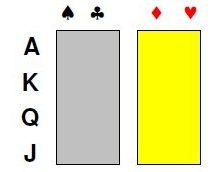
\includegraphics[width=1\linewidth,height=\textheight,keepaspectratio]{../../images/AA/barsit3.jpg}

}

\subcaption{Agrupar por cor do naipe?}

\end{figure}%

\end{minipage}%
%
\begin{minipage}{0.50\linewidth}

\begin{figure}[H]

{\centering 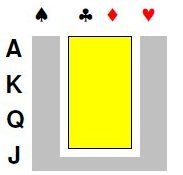
\includegraphics[width=0.8\linewidth,height=\textheight,keepaspectratio]{../../images/AA/barsit4.jpg}

}

\subcaption{Agrupar por naipes maiores e menores?}

\end{figure}%

\end{minipage}%

\end{figure}%
\end{frame}

\begin{frame}{Algumas questões\ldots{}}
\phantomsection\label{algumas-questuxf5es-4}
\begin{figure}

\begin{minipage}{0.50\linewidth}

\begin{figure}[H]

{\centering 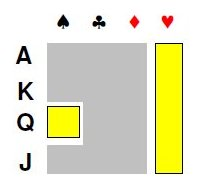
\includegraphics[width=0.85\linewidth,height=\textheight,keepaspectratio]{../../images/AA/barsit5.jpg}

}

\subcaption{Copas mais a Rainha de espadas e outros naipes?}

\end{figure}%

\end{minipage}%
%
\begin{minipage}{0.50\linewidth}

\begin{figure}[H]

{\centering 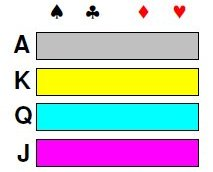
\includegraphics[width=0.96\linewidth,height=\textheight,keepaspectratio]{../../images/AA/barsit6.jpg}

}

\subcaption{Agrupar por face da carta?}

\end{figure}%

\end{minipage}%

\end{figure}%
\end{frame}

\begin{frame}{Algumas questões\ldots{}}
\phantomsection\label{algumas-questuxf5es-5}
\begin{block}{Resumindo\ldots{}}
\phantomsection\label{resumindo}
\textbf{Necessidade} da definição de medidas de \textbf{similaridade}
(ou dissimilaridade)

\begin{center}
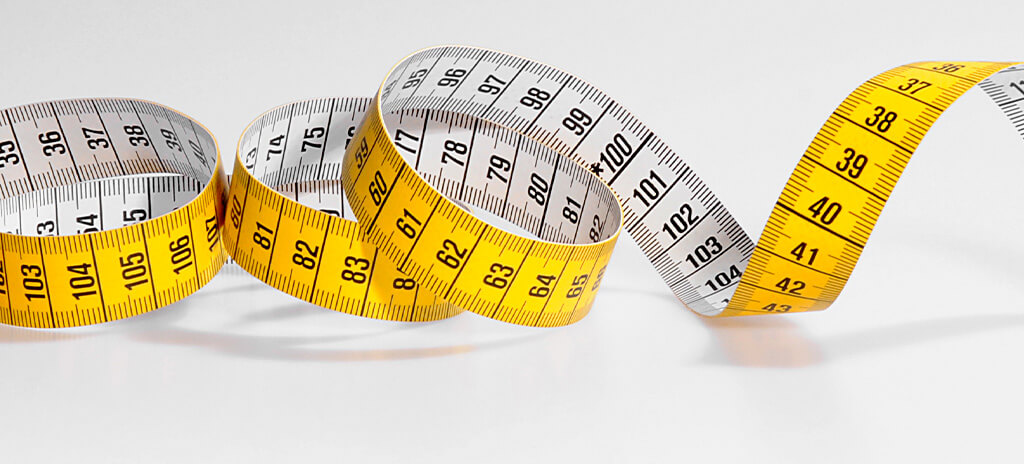
\includegraphics[width=1\linewidth,height=\textheight,keepaspectratio]{../../images/AA/medidas.jpg}
\end{center}
\end{block}
\end{frame}

\begin{frame}{Similaridade e dissimilaridade}
\phantomsection\label{similaridade-e-dissimilaridade}
\textbf{Medidas de Similaridade:} quanto \textbf{maior} o valor,
\textbf{maior a semelhança} entre os objetos

\pause

\textbf{Medidas de Dissimilaridade (Distância):} quanto \textbf{maior} o
valor, \textbf{mais diferentes} são os objetos
\end{frame}

\begin{frame}{Similaridade e dissimilaridade (exemplo)}
\phantomsection\label{similaridade-e-dissimilaridade-exemplo}
\textbf{Pesquisa com clientes de uma loja de equipamentos automotivos}

\pause

\textbf{Variáveis mensuradas}

\begin{itemize}
\item
  \textbf{Idade} (em anos completos) - Variável quantitativa discreta
\item
  \textbf{Número de carros} - Variável quantitativa discreta
\item
  \textbf{Classe social}: A, B, C ou D - Variável qualitativa ordinal
\item
  \textbf{Potência do motor}: Baixa, Média ou Alta - Variável
  qualitativa ordinal
\item
  \textbf{Combustível}: Gasolina ou Álcool - Variável qualitativa
  nominal
\item
  \textbf{Modelo}: Esporte, Luxo ou Standard - Variável qualitativa
  nominal
\end{itemize}
\end{frame}

\begin{frame}{Base de dados (exemplo)}
\phantomsection\label{base-de-dados-exemplo}
\begin{longtable}[]{@{}
  >{\raggedleft\arraybackslash}p{(\linewidth - 12\tabcolsep) * \real{0.0849}}
  >{\raggedleft\arraybackslash}p{(\linewidth - 12\tabcolsep) * \real{0.1038}}
  >{\raggedleft\arraybackslash}p{(\linewidth - 12\tabcolsep) * \real{0.1792}}
  >{\raggedright\arraybackslash}p{(\linewidth - 12\tabcolsep) * \real{0.1792}}
  >{\raggedright\arraybackslash}p{(\linewidth - 12\tabcolsep) * \real{0.2075}}
  >{\raggedright\arraybackslash}p{(\linewidth - 12\tabcolsep) * \real{0.1415}}
  >{\raggedright\arraybackslash}p{(\linewidth - 12\tabcolsep) * \real{0.1038}}@{}}
\toprule\noalign{}
\begin{minipage}[b]{\linewidth}\raggedleft
Cliente
\end{minipage} & \begin{minipage}[b]{\linewidth}\raggedleft
\textbf{Idade}
\end{minipage} & \begin{minipage}[b]{\linewidth}\raggedleft
\textbf{N.º de carros}
\end{minipage} & \begin{minipage}[b]{\linewidth}\raggedright
\textbf{Classe social}
\end{minipage} & \begin{minipage}[b]{\linewidth}\raggedright
\textbf{Potência do motor}
\end{minipage} & \begin{minipage}[b]{\linewidth}\raggedright
\textbf{Combustível}
\end{minipage} & \begin{minipage}[b]{\linewidth}\raggedright
\textbf{Modelo}
\end{minipage} \\
\midrule\noalign{}
\endhead
1 & 20 & 1 & A & Baixa & Gasolina & Esporte \\
2 & 37 & 2 & A & Alta & Gasolina & Luxo \\
3 & 51 & 1 & C & Média & Gasolina & Esporte \\
4 & 32 & 1 & D & Alta & Álcool & Standard \\
5 & 30 & 2 & B & Média & Álcool & Standard \\
6 & 55 & 3 & A & Alta & Gasolina & Luxo \\
\bottomrule\noalign{}
\end{longtable}

\pause

\textbf{Como medir a similaridade ou dissimilaridade entre os
indivíduos?}
\end{frame}

\section{Variáveis quantitativas}\label{variuxe1veis-quantitativas}

\begin{frame}{Dissimilaridade}
\phantomsection\label{dissimilaridade}
As \textbf{distâncias} são as medidas de \textbf{dissimilaridade} mais
utilizadas no estudo de bancos de dados com variáveis numéricas

\pause

\begin{itemize}
\tightlist
\item
  Uma medida \(d_{ij}\) representa uma \textbf{medida de distância}
  entre os indivíduos \(i\) e \(j\) se, e somente se,

  \begin{enumerate}
  [a)]
  \tightlist
  \item
    \(d_{ij} \geqslant 0\) para todo \(i\) e \(j\);
  \item
    \(d_{ij} = 0\) se, e somente se, \(i = j\);
  \item
    \(d_{ij} = d_{ji}\)
  \item
    \(d_{ij} \leqslant d_{ik} + d_{kj}\) para qualquer indivíduo \(k\).
  \end{enumerate}
\end{itemize}
\end{frame}

\begin{frame}{Dissimilaridade}
\phantomsection\label{dissimilaridade-1}
\begin{figure}[H]

{\centering 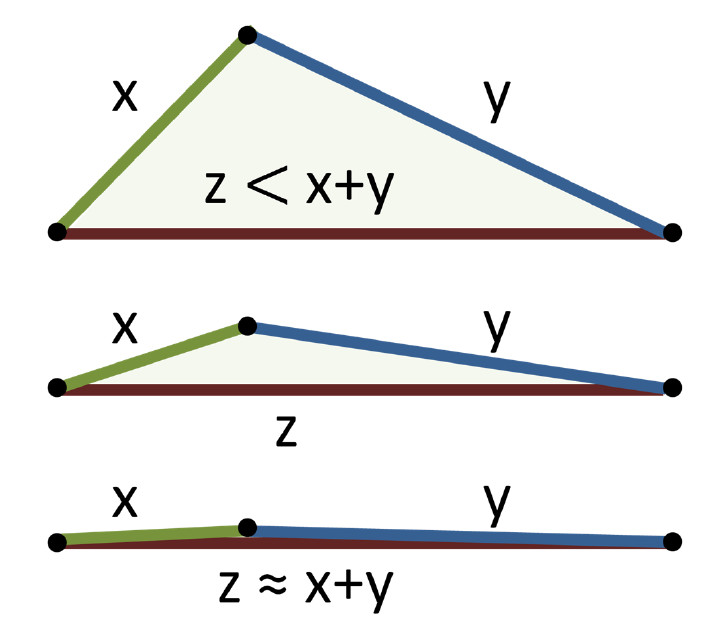
\includegraphics[width=1\linewidth,height=\textheight,keepaspectratio]{../../images/AA/desig_tri.jpg}

}

\caption{Desigualdade triangular}

\end{figure}%
\end{frame}

\begin{frame}{Dissimilaridade}
\phantomsection\label{dissimilaridade-2}
\begin{block}{Principais medidas de distância}
\phantomsection\label{principais-medidas-de-distuxe2ncia}
\textbf{Distância Euclidiana}

\[d_{ij} = \displaystyle{\sqrt{(\mathbf{x}_i - \mathbf{x}_j)^t(\mathbf{x}_i - \mathbf{x}_j)}} = \sqrt{\displaystyle{\sum_{k=1}^p(x_{ik} - x_{jk})^2}}\]

Distância geométrica entre dois pontos
\end{block}
\end{frame}

\begin{frame}{Dissimilaridade}
\phantomsection\label{dissimilaridade-3}
\begin{block}{Principais medidas de distância}
\phantomsection\label{principais-medidas-de-distuxe2ncia-1}
\textbf{Distância Euclidiana Generalizada}

\[d_{ij} = \displaystyle{\sqrt{(\mathbf{x}_i - \mathbf{x}_j)^t\boldsymbol{W}(\mathbf{x}_i - \mathbf{x}_j)}}\]

\begin{itemize}
\item
  Se \(\boldsymbol{W} = \textrm{diag}\left(\dfrac{1}{p}\right)\):
  \textbf{distância euclidiana média}
\item
  Se \(\boldsymbol{W} = \boldsymbol{\Sigma}^{-1}\): \textbf{distância de
  Mahalanobis}
\end{itemize}
\end{block}
\end{frame}

\begin{frame}{Dissimilaridade}
\phantomsection\label{dissimilaridade-4}
\begin{block}{Principais medidas de distância}
\phantomsection\label{principais-medidas-de-distuxe2ncia-2}
\textbf{Distância de Minkowski}

\[d_{ij} = \left( \displaystyle{\sum_{k=1}^P} |X_{ik} - X_{jk}|^{\lambda}\right)^{\frac{1}{\lambda}}\]

\begin{itemize}
\tightlist
\item
  Se \(\lambda = 1\), temos a chamada \textbf{métrica de Manhattan}. É
  também conhecida como \emph{city block}.\\
\item
  Se \(\lambda = 2\), temos a distância euclidiana.
\item
  A métrica de Minkowski é menos afetada pela presença de valores
  discrepantes na amostra do que a distância Euclidiana.
\end{itemize}
\end{block}
\end{frame}

\begin{frame}{Dissimilaridade}
\phantomsection\label{dissimilaridade-5}
\begin{block}{Principais medidas de distância}
\phantomsection\label{principais-medidas-de-distuxe2ncia-3}
\textbf{Distância de Manhattan (city block)}

\begin{center}
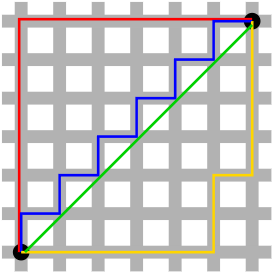
\includegraphics[width=1\linewidth,height=\textheight,keepaspectratio]{../../images/AA/cityblock.png}
\end{center}
\end{block}
\end{frame}

\begin{frame}{Dissimilaridade}
\phantomsection\label{dissimilaridade-6}
\begin{block}{Dissimilaridade \(\Longrightarrow\) Similaridade}
\phantomsection\label{dissimilaridade-longrightarrow-similaridade}
\[s_{ij} = 1 - d_{ij}^0\]

em que

\[d_{ij}^0 = \displaystyle{\frac{d_{ij} - \min(\boldsymbol{D})}{\max(\boldsymbol{D}) - \min(\boldsymbol{D})}}\]

Sendo \(\min(\boldsymbol{D})\) e \(\max(\boldsymbol{D})\) o menor e o
maior valor de distância observados na matriz de distâncias
\(\boldsymbol{D}_{n \times n}\), sem levar em consideração os elementos
da diagonal principal dessa matriz.
\end{block}
\end{frame}

\section{Variáveis qualitativas}\label{variuxe1veis-qualitativas}

\begin{frame}{Similaridade}
\phantomsection\label{similaridade}
\begin{block}{Variáveis qualitativas nominais}
\phantomsection\label{variuxe1veis-qualitativas-nominais}
Neste caso, utilizamos variáveis fictícias (variáveis \emph{dummy}) para
\textbf{codificar} as variáveis:

\begin{columns}[T]
\begin{column}{0.5\linewidth}
\begin{longtable}[]{@{}lr@{}}
\toprule\noalign{}
Combustível & \(N_1\) \\
\midrule\noalign{}
\endhead
Gasolina & 1 \\
Álcool & 0 \\
\bottomrule\noalign{}
\end{longtable}
\end{column}

\begin{column}{0.5\linewidth}
\begin{longtable}[]{@{}lrr@{}}
\toprule\noalign{}
Modelo & \(N_2\) & \(N_3\) \\
\midrule\noalign{}
\endhead
Esporte & 1 & 0 \\
Luxo & 0 & 1 \\
Standard & 0 & 0 \\
\bottomrule\noalign{}
\end{longtable}
\end{column}
\end{columns}
\end{block}
\end{frame}

\begin{frame}{Similaridade}
\phantomsection\label{similaridade-1}
\begin{block}{Variáveis qualitativas nominais}
\phantomsection\label{variuxe1veis-qualitativas-nominais-1}
\textbf{No exemplo:}

\begin{columns}[T]
\begin{column}{0.5\linewidth}
\begin{longtable}[]{@{}rlr@{}}
\toprule\noalign{}
Cliente & Combustível & \(N_1\) \\
\midrule\noalign{}
\endhead
1 & Gasolina & 1 \\
2 & Gasolina & 1 \\
3 & Gasolina & 1 \\
4 & Álcool & 0 \\
5 & Álcool & 0 \\
6 & Gasolina & 1 \\
\bottomrule\noalign{}
\end{longtable}
\end{column}

\begin{column}{0.5\linewidth}
\begin{longtable}[]{@{}rlrr@{}}
\toprule\noalign{}
Cliente & Modelo & \(N_2\) & \(N_3\) \\
\midrule\noalign{}
\endhead
1 & Esporte & 1 & 0 \\
2 & Luxo & 0 & 1 \\
3 & Esporte & 1 & 0 \\
4 & Standard & 0 & 0 \\
5 & Standard & 0 & 0 \\
6 & Luxo & 0 & 1 \\
\bottomrule\noalign{}
\end{longtable}
\end{column}
\end{columns}
\end{block}
\end{frame}

\begin{frame}{Similaridade}
\phantomsection\label{similaridade-2}
\begin{block}{Variáveis qualitativas nominais}
\phantomsection\label{variuxe1veis-qualitativas-nominais-2}
De forma que,

\begin{longtable}[]{@{}rrrr@{}}
\toprule\noalign{}
Cliente & \(N_1\) & \(N_2\) & \(N_3\) \\
\midrule\noalign{}
\endhead
1 & 1 & 1 & 0 \\
2 & 1 & 0 & 1 \\
3 & 1 & 1 & 0 \\
4 & 0 & 0 & 0 \\
5 & 0 & 0 & 0 \\
6 & 1 & 0 & 1 \\
\bottomrule\noalign{}
\end{longtable}
\end{block}
\end{frame}

\begin{frame}{Similaridade}
\phantomsection\label{similaridade-3}
\begin{block}{Variáveis qualitativas ordinais}
\phantomsection\label{variuxe1veis-qualitativas-ordinais}
Utilizamos variáveis fictícias (variáveis \emph{dummy}) para
\textbf{codificar} as variáveis, levando em consideração a ordinalidade
das variáveis:

\begin{columns}[T]
\begin{column}{0.5\linewidth}
\begin{longtable}[]{@{}lrrr@{}}
\toprule\noalign{}
Classe social & \(O_1\) & \(O_2\) & \(O_3\) \\
\midrule\noalign{}
\endhead
A & 1 & 1 & 1 \\
B & 0 & 1 & 1 \\
C & 0 & 0 & 1 \\
D & 0 & 0 & 0 \\
\bottomrule\noalign{}
\end{longtable}
\end{column}

\begin{column}{0.5\linewidth}
\begin{longtable}[]{@{}lrr@{}}
\toprule\noalign{}
Potência & \(O_4\) & \(O_5\) \\
\midrule\noalign{}
\endhead
Alta & 1 & 1 \\
Média & 0 & 1 \\
Baixa & 0 & 0 \\
\bottomrule\noalign{}
\end{longtable}
\end{column}
\end{columns}
\end{block}
\end{frame}

\begin{frame}{Similaridade}
\phantomsection\label{similaridade-4}
\begin{block}{Observação}
\phantomsection\label{observauxe7uxe3o}
As variáveis \textbf{Classe social} e \textbf{Potência do motor} possuem
\textbf{ordem natural}. Por isso, foram codificadas por meio de
\textbf{variáveis ordinais cumulativas}:

\begin{itemize}
\tightlist
\item
  valores mais altos acumulam mais indicadores iguais a 1;
\item
  valores mais baixos recebem apenas zeros.
\end{itemize}

Essa codificação preserva a informação de ordem, mas impõe uma estrutura
geométrica específica ao espaço dos dados.
\end{block}
\end{frame}

\begin{frame}{Similaridade}
\phantomsection\label{similaridade-5}
\begin{block}{Variáveis qualitativas ordinais}
\phantomsection\label{variuxe1veis-qualitativas-ordinais-1}
\textbf{No exemplo:}

\begin{columns}[T]
\begin{column}{0.5\linewidth}
\begin{longtable}[]{@{}rlrrr@{}}
\toprule\noalign{}
Cliente & Classe social & \(O_1\) & \(O_2\) & \(O_3\) \\
\midrule\noalign{}
\endhead
1 & A & 1 & 1 & 1 \\
2 & A & 1 & 1 & 1 \\
3 & C & 0 & 0 & 1 \\
4 & D & 0 & 0 & 0 \\
5 & B & 0 & 1 & 1 \\
6 & A & 1 & 1 & 1 \\
\bottomrule\noalign{}
\end{longtable}
\end{column}

\begin{column}{0.5\linewidth}
\begin{longtable}[]{@{}rlrr@{}}
\toprule\noalign{}
Cliente & Potência & \(O_4\) & \(O_5\) \\
\midrule\noalign{}
\endhead
1 & Baixa & 0 & 0 \\
2 & Alta & 1 & 1 \\
3 & Média & 0 & 1 \\
4 & Alta & 1 & 1 \\
5 & Média & 0 & 1 \\
6 & Alta & 1 & 1 \\
\bottomrule\noalign{}
\end{longtable}
\end{column}
\end{columns}
\end{block}
\end{frame}

\begin{frame}{Similaridade}
\phantomsection\label{similaridade-6}
\begin{block}{Variáveis qualitativas ordinais}
\phantomsection\label{variuxe1veis-qualitativas-ordinais-2}
De forma que,

\begin{longtable}[]{@{}rrrrrr@{}}
\toprule\noalign{}
Cliente & \(O_1\) & \(O_2\) & \(O_3\) & \(O_4\) & \(O_5\) \\
\midrule\noalign{}
\endhead
1 & 1 & 1 & 1 & 0 & 0 \\
2 & 1 & 1 & 1 & 1 & 1 \\
3 & 0 & 0 & 1 & 0 & 1 \\
4 & 0 & 0 & 0 & 1 & 1 \\
5 & 0 & 1 & 1 & 0 & 1 \\
6 & 1 & 1 & 1 & 1 & 1 \\
\bottomrule\noalign{}
\end{longtable}
\end{block}
\end{frame}

\begin{frame}{Similaridade}
\phantomsection\label{similaridade-7}
\begin{block}{Variáveis qualitativas nominais e ordinais}
\phantomsection\label{variuxe1veis-qualitativas-nominais-e-ordinais}
Juntando tudo\ldots{}

\begin{longtable}[]{@{}
  >{\raggedleft\arraybackslash}p{(\linewidth - 16\tabcolsep) * \real{0.1385}}
  >{\raggedleft\arraybackslash}p{(\linewidth - 16\tabcolsep) * \real{0.1077}}
  >{\raggedleft\arraybackslash}p{(\linewidth - 16\tabcolsep) * \real{0.1077}}
  >{\raggedleft\arraybackslash}p{(\linewidth - 16\tabcolsep) * \real{0.1077}}
  >{\raggedleft\arraybackslash}p{(\linewidth - 16\tabcolsep) * \real{0.1077}}
  >{\raggedleft\arraybackslash}p{(\linewidth - 16\tabcolsep) * \real{0.1077}}
  >{\raggedleft\arraybackslash}p{(\linewidth - 16\tabcolsep) * \real{0.1077}}
  >{\raggedleft\arraybackslash}p{(\linewidth - 16\tabcolsep) * \real{0.1077}}
  >{\raggedleft\arraybackslash}p{(\linewidth - 16\tabcolsep) * \real{0.1077}}@{}}
\toprule\noalign{}
\begin{minipage}[b]{\linewidth}\raggedleft
Cliente
\end{minipage} & \begin{minipage}[b]{\linewidth}\raggedleft
\(O_1\)
\end{minipage} & \begin{minipage}[b]{\linewidth}\raggedleft
\(O_2\)
\end{minipage} & \begin{minipage}[b]{\linewidth}\raggedleft
\(O_3\)
\end{minipage} & \begin{minipage}[b]{\linewidth}\raggedleft
\(O_4\)
\end{minipage} & \begin{minipage}[b]{\linewidth}\raggedleft
\(O_5\)
\end{minipage} & \begin{minipage}[b]{\linewidth}\raggedleft
\(N_1\)
\end{minipage} & \begin{minipage}[b]{\linewidth}\raggedleft
\(N_2\)
\end{minipage} & \begin{minipage}[b]{\linewidth}\raggedleft
\(N_3\)
\end{minipage} \\
\midrule\noalign{}
\endhead
1 & 1 & 1 & 1 & 0 & 0 & 1 & 1 & 0 \\
2 & 1 & 1 & 1 & 1 & 1 & 1 & 0 & 1 \\
3 & 0 & 0 & 1 & 0 & 1 & 1 & 1 & 0 \\
4 & 0 & 0 & 0 & 1 & 1 & 0 & 0 & 0 \\
5 & 0 & 1 & 1 & 0 & 1 & 0 & 0 & 0 \\
6 & 1 & 1 & 1 & 1 & 1 & 1 & 0 & 1 \\
\bottomrule\noalign{}
\end{longtable}
\end{block}
\end{frame}

\begin{frame}{Similaridade}
\phantomsection\label{similaridade-8}
\begin{block}{Variáveis qualitativas nominais e ordinais}
\phantomsection\label{variuxe1veis-qualitativas-nominais-e-ordinais-1}
Considere os clientes 1 e 3. Vamos calcular a medida de similaridade
entre eles:

\begin{longtable}[]{@{}
  >{\raggedleft\arraybackslash}p{(\linewidth - 16\tabcolsep) * \real{0.1385}}
  >{\raggedleft\arraybackslash}p{(\linewidth - 16\tabcolsep) * \real{0.1077}}
  >{\raggedleft\arraybackslash}p{(\linewidth - 16\tabcolsep) * \real{0.1077}}
  >{\raggedleft\arraybackslash}p{(\linewidth - 16\tabcolsep) * \real{0.1077}}
  >{\raggedleft\arraybackslash}p{(\linewidth - 16\tabcolsep) * \real{0.1077}}
  >{\raggedleft\arraybackslash}p{(\linewidth - 16\tabcolsep) * \real{0.1077}}
  >{\raggedleft\arraybackslash}p{(\linewidth - 16\tabcolsep) * \real{0.1077}}
  >{\raggedleft\arraybackslash}p{(\linewidth - 16\tabcolsep) * \real{0.1077}}
  >{\raggedleft\arraybackslash}p{(\linewidth - 16\tabcolsep) * \real{0.1077}}@{}}
\toprule\noalign{}
\begin{minipage}[b]{\linewidth}\raggedleft
Cliente
\end{minipage} & \begin{minipage}[b]{\linewidth}\raggedleft
\(O_1\)
\end{minipage} & \begin{minipage}[b]{\linewidth}\raggedleft
\(O_2\)
\end{minipage} & \begin{minipage}[b]{\linewidth}\raggedleft
\(O_3\)
\end{minipage} & \begin{minipage}[b]{\linewidth}\raggedleft
\(O_4\)
\end{minipage} & \begin{minipage}[b]{\linewidth}\raggedleft
\(O_5\)
\end{minipage} & \begin{minipage}[b]{\linewidth}\raggedleft
\(N_1\)
\end{minipage} & \begin{minipage}[b]{\linewidth}\raggedleft
\(N_2\)
\end{minipage} & \begin{minipage}[b]{\linewidth}\raggedleft
\(N_3\)
\end{minipage} \\
\midrule\noalign{}
\endhead
1 & 1 & 1 & 1 & 0 & 0 & 1 & 1 & 0 \\
3 & 0 & 0 & 1 & 0 & 1 & 1 & 1 & 0 \\
\bottomrule\noalign{}
\end{longtable}
\end{block}
\end{frame}

\begin{frame}{Similaridade}
\phantomsection\label{similaridade-9}
\begin{block}{Tabela de concordância entre dois indivíduos}
\phantomsection\label{tabela-de-concorduxe2ncia-entre-dois-indivuxedduos}
\begin{longtable}[]{@{}llll@{}}
\toprule\noalign{}
Indivíduo \(i\) \textbackslash{} Indivíduo \(j\) & 1 & 0 & Total \\
\midrule\noalign{}
\endhead
1 & \(a\) & \(b\) & \(a + b\) \\
0 & \(c\) & \(d\) & \(c + d\) \\
\textbf{Total} & \(a + c\) & \(b + d\) & \(p\) \\
\bottomrule\noalign{}
\end{longtable}

\begin{itemize}
\tightlist
\item
  \(a\): número de variáveis em que ambos têm valor 1
\item
  \(b\): número de variáveis em que \(i=1\) e \(j=0\)
\item
  \(c\): número de variáveis em que \(i=0\) e \(j=1\)
\item
  \(d\): número de variáveis em que ambos têm valor 0
\end{itemize}

\[p = a + b + c + d\]
\end{block}
\end{frame}

\begin{frame}{Similaridade}
\phantomsection\label{similaridade-10}
\begin{block}{Tabela de concordância entre dois indivíduos}
\phantomsection\label{tabela-de-concorduxe2ncia-entre-dois-indivuxedduos-1}
\textbf{No exemplo:}

\begin{longtable}[]{@{}llll@{}}
\toprule\noalign{}
Indivíduo 1 \textbackslash{} Indivíduo 3 & 1 & 0 & Total \\
\midrule\noalign{}
\endhead
1 & 3 & 2 & 5 \\
0 & 1 & 2 & 3 \\
\textbf{Total} & 4 & 4 & 8 \\
\bottomrule\noalign{}
\end{longtable}
\end{block}
\end{frame}

\section{\texorpdfstring{Como extrair as \textbf{medidas de
similaridade} baseadas na \textbf{tabela de concordância} dos
elementos?}{Como extrair as medidas de similaridade baseadas na tabela de concordância dos elementos?}}\label{como-extrair-as-medidas-de-similaridade-baseadas-na-tabela-de-concorduxe2ncia-dos-elementos}

\begin{frame}{Critérios de similaridade}
\phantomsection\label{crituxe9rios-de-similaridade}
\begin{block}{Coeficiente de Concordância Simples}
\phantomsection\label{coeficiente-de-concorduxe2ncia-simples}
\[\Large s_{ij} = \displaystyle{\frac{a + d}{p}}\]

\begin{columns}[T]
\begin{column}{0.5\linewidth}
\begin{longtable}[]{@{}llll@{}}
\toprule\noalign{}
Indivíduo 1 \textbackslash{} Indivíduo 3 & 1 & 0 & Total \\
\midrule\noalign{}
\endhead
1 & 3 & 2 & 5 \\
0 & 1 & 2 & 3 \\
\textbf{Total} & 4 & 4 & 8 \\
\bottomrule\noalign{}
\end{longtable}
\end{column}

\begin{column}{0.5\linewidth}
\[
s_{13} = \dfrac{a + d}{p}
               = \dfrac{3 + 2}{8}
               = \dfrac{5}{8}
               = 0,625
\]
\end{column}
\end{columns}
\end{block}
\end{frame}

\begin{frame}{Critérios de similaridade}
\phantomsection\label{crituxe9rios-de-similaridade-1}
\begin{block}{Coeficiente de Concordância Simples}
\phantomsection\label{coeficiente-de-concorduxe2ncia-simples-1}
\textbf{Interpretação:}

\begin{itemize}
\item
  O valor 0,625 indica que os indivíduos 1 e 3 concordam em 62,5\% das
  variáveis binárias.
\item
  Tanto concordâncias em 1 quanto em 0 contribuem igualmente para a
  similaridade.
\end{itemize}
\end{block}
\end{frame}

\begin{frame}{Critérios de similaridade}
\phantomsection\label{crituxe9rios-de-similaridade-2}
\begin{block}{Coeficiente de Concordância Positiva}
\phantomsection\label{coeficiente-de-concorduxe2ncia-positiva}
\[\Large s_{ij} = \displaystyle{\frac{a}{p}}\]

\begin{columns}[T]
\begin{column}{0.5\linewidth}
\begin{longtable}[]{@{}llll@{}}
\toprule\noalign{}
Indivíduo 1 \textbackslash{} Indivíduo 3 & 1 & 0 & Total \\
\midrule\noalign{}
\endhead
1 & 3 & 2 & 5 \\
0 & 1 & 2 & 3 \\
\textbf{Total} & 4 & 4 & 8 \\
\bottomrule\noalign{}
\end{longtable}
\end{column}

\begin{column}{0.5\linewidth}
\[
s_{13} = \dfrac{a}{p}= 
               \dfrac{3}{8} = 0,375
\]
\end{column}
\end{columns}
\end{block}
\end{frame}

\begin{frame}{Critérios de similaridade}
\phantomsection\label{crituxe9rios-de-similaridade-3}
\begin{block}{Coeficiente de Concordância Positiva}
\phantomsection\label{coeficiente-de-concorduxe2ncia-positiva-1}
\textbf{Interpretação:}

\begin{itemize}
\tightlist
\item
  Os indivíduos 1 e 3 compartilham simultaneamente o valor 1 em
  \textbf{37,5\%} das variáveis.
\item
  Ausências simultâneas (valor 0) \textbf{não contribuem} para a
  similaridade.
\item
  O critério enfatiza \textbf{presença conjunta}, não coincidência
  geral.
\end{itemize}
\end{block}
\end{frame}

\begin{frame}{Critérios de similaridade}
\phantomsection\label{crituxe9rios-de-similaridade-4}
\begin{block}{Coeficiente de Concordância de Jaccard}
\phantomsection\label{coeficiente-de-concorduxe2ncia-de-jaccard}
\[\Large s_{ij} = \displaystyle{\frac{a}{a + b + c}}\]

\begin{columns}[T]
\begin{column}{0.5\linewidth}
\begin{longtable}[]{@{}llll@{}}
\toprule\noalign{}
Indivíduo 1 \textbackslash{} Indivíduo 3 & 1 & 0 & Total \\
\midrule\noalign{}
\endhead
1 & 3 & 2 & 5 \\
0 & 1 & 2 & 3 \\
\textbf{Total} & 4 & 4 & 8 \\
\bottomrule\noalign{}
\end{longtable}
\end{column}

\begin{column}{0.5\linewidth}
\[
s_{13} = \dfrac{3}{3 + 2 + 1}
       = \dfrac{3}{6}
       = 0,5
\]
\end{column}
\end{columns}
\end{block}
\end{frame}

\begin{frame}{Critérios de similaridade}
\phantomsection\label{crituxe9rios-de-similaridade-5}
\begin{block}{Coeficiente de Concordância de Jaccard}
\phantomsection\label{coeficiente-de-concorduxe2ncia-de-jaccard-1}
\textbf{Interpretação:}

\begin{itemize}
\tightlist
\item
  Os indivíduos 1 e 3 compartilham \textbf{50\% das presenças
  observadas}.
\item
  Ausências simultâneas (valor 0) \textbf{não contribuem} para a
  similaridade.
\item
  O coeficiente foca exclusivamente na \textbf{interseção de atributos
  presentes}.
\end{itemize}
\end{block}
\end{frame}

\begin{frame}{Critérios de similaridade}
\phantomsection\label{crituxe9rios-de-similaridade-6}
\begin{block}{Coeficiente de Concordância de Gower e Legendre}
\phantomsection\label{coeficiente-de-concorduxe2ncia-de-gower-e-legendre}
O \textbf{Coeficiente de Concordância de Gower--Legendre} é uma medida
de similaridade projetada para \textbf{dados mistos}, isto é, conjuntos
de dados que contêm, ao mesmo tempo:

\begin{itemize}
\tightlist
\item
  variáveis quantitativas,
\item
  variáveis qualitativas nominais,
\item
  variáveis qualitativas ordinais.
\end{itemize}

Ele permite combinar diferentes tipos de variáveis em \textbf{uma única
medida de similaridade}, respeitando a natureza de cada uma.
\end{block}
\end{frame}

\begin{frame}{Critérios de similaridade}
\phantomsection\label{crituxe9rios-de-similaridade-7}
\begin{block}{Coeficiente de Concordância de Gower e Legendre}
\phantomsection\label{coeficiente-de-concorduxe2ncia-de-gower-e-legendre-1}
Considere dois indivíduos \(i\) e \(j\) descritos por \(p\) variáveis. A
similaridade de Gower--Legendre é definida como:

\[
S_{ij}
=
\dfrac{\sum_{k=1}^{p} w_{ijk}\, s_{ijk}}
{\sum_{k=1}^{p} w_{ijk}},
\] onde:

\begin{itemize}
\tightlist
\item
  \(s_{ijk}\) é a similaridade parcial da variável \(k\) entre os
  indivíduos \(i\) e \(j\);
\item
  \(w_{ijk}\) é um peso (geralmente \(0\) ou \(1\)), usado para tratar
  dados ausentes.
\end{itemize}
\end{block}
\end{frame}

\begin{frame}{Critérios de similaridade}
\phantomsection\label{crituxe9rios-de-similaridade-8}
\begin{block}{Coeficiente de Concordância de Gower e Legendre}
\phantomsection\label{coeficiente-de-concorduxe2ncia-de-gower-e-legendre-2}
O coeficiente assume valores em \([0,1]\):

\begin{itemize}
\tightlist
\item
  \(S_{ij} = 1\) indica indivíduos idênticos;
\item
  \(S_{ij} = 0\) indica máxima dissimilaridade.
\end{itemize}
\end{block}
\end{frame}

\begin{frame}{Critérios de similaridade}
\phantomsection\label{crituxe9rios-de-similaridade-9}
\begin{block}{Coeficiente de Concordância de Gower e Legendre}
\phantomsection\label{coeficiente-de-concorduxe2ncia-de-gower-e-legendre-3}
\begin{block}{Similaridade parcial por tipo de variável}
\phantomsection\label{similaridade-parcial-por-tipo-de-variuxe1vel}
\textbf{Variáveis quantitativas}

\begin{itemize}
\tightlist
\item
  Para uma variável quantitativa \(k\):
\end{itemize}

\[
s_{ijk}
=
1 - \dfrac{|x_{ik} - x_{jk}|}{R_k},
\]

onde \(R_k\) é o intervalo da variável \(k\) (máximo − mínimo).
\end{block}
\end{block}
\end{frame}

\begin{frame}{Critérios de similaridade}
\phantomsection\label{crituxe9rios-de-similaridade-10}
\begin{block}{Coeficiente de Concordância de Gower e Legendre}
\phantomsection\label{coeficiente-de-concorduxe2ncia-de-gower-e-legendre-4}
\begin{block}{Similaridade parcial por tipo de variável}
\phantomsection\label{similaridade-parcial-por-tipo-de-variuxe1vel-1}
\textbf{Variáveis qualitativas nominais}

\begin{itemize}
\tightlist
\item
  Para uma variável nominal:
\end{itemize}

\[
s_{ijk}
=
\begin{cases}
1, & \text{se } x_{ik} = x_{jk}, \\
0, & \text{caso contrário}.
\end{cases}
\]
\end{block}
\end{block}
\end{frame}

\begin{frame}{Critérios de similaridade}
\phantomsection\label{crituxe9rios-de-similaridade-11}
\begin{block}{Coeficiente de Concordância de Gower e Legendre}
\phantomsection\label{coeficiente-de-concorduxe2ncia-de-gower-e-legendre-5}
\begin{block}{Similaridade parcial por tipo de variável}
\phantomsection\label{similaridade-parcial-por-tipo-de-variuxe1vel-2}
\textbf{Variáveis qualitativas ordinais}

Para variáveis ordinais, os níveis são primeiro convertidos em
\textbf{postos normalizados} no intervalo \([0,1]\). Em seguida,
aplica-se a mesma fórmula das variáveis quantitativas:

\[
s_{ijk}
=
1 - |r_{ik} - r_{jk}|,
\]

onde \(r_{ik}\) e \(r_{jk}\) são os postos normalizados.
\end{block}
\end{block}
\end{frame}

\begin{frame}{Critérios de similaridade}
\phantomsection\label{crituxe9rios-de-similaridade-12}
\begin{block}{Coeficiente de Concordância de Gower e Legendre}
\phantomsection\label{coeficiente-de-concorduxe2ncia-de-gower-e-legendre-6}
\textbf{Interpretação:}

\begin{itemize}
\tightlist
\item
  Cada variável contribui \textbf{de forma controlada} para a
  similaridade total.
\item
  Variáveis com escalas diferentes \textbf{não dominam} o cálculo.
\item
  A ordem das categorias é respeitada para variáveis ordinais,
  \textbf{sem impor distâncias artificiais}.
\end{itemize}
\end{block}
\end{frame}

\begin{frame}{Critérios de similaridade}
\phantomsection\label{crituxe9rios-de-similaridade-13}
\begin{block}{Similaridade \(\Longrightarrow\) Dissimilaridade}
\phantomsection\label{similaridade-longrightarrow-dissimilaridade}
\[\Large d_{ij}^* = 1 - s_{ij}\]
\end{block}
\end{frame}

\begin{frame}{Critérios de similaridade}
\phantomsection\label{crituxe9rios-de-similaridade-14}
\begin{block}{Coeficiente de Concordância de Gower e Legendre}
\phantomsection\label{coeficiente-de-concorduxe2ncia-de-gower-e-legendre-7}
\textbf{No exemplo:}

\begin{longtable}[]{@{}
  >{\raggedleft\arraybackslash}p{(\linewidth - 12\tabcolsep) * \real{0.0849}}
  >{\raggedleft\arraybackslash}p{(\linewidth - 12\tabcolsep) * \real{0.1038}}
  >{\raggedleft\arraybackslash}p{(\linewidth - 12\tabcolsep) * \real{0.1792}}
  >{\raggedright\arraybackslash}p{(\linewidth - 12\tabcolsep) * \real{0.1792}}
  >{\raggedright\arraybackslash}p{(\linewidth - 12\tabcolsep) * \real{0.2075}}
  >{\raggedright\arraybackslash}p{(\linewidth - 12\tabcolsep) * \real{0.1415}}
  >{\raggedright\arraybackslash}p{(\linewidth - 12\tabcolsep) * \real{0.1038}}@{}}
\toprule\noalign{}
\begin{minipage}[b]{\linewidth}\raggedleft
Cliente
\end{minipage} & \begin{minipage}[b]{\linewidth}\raggedleft
\textbf{Idade}
\end{minipage} & \begin{minipage}[b]{\linewidth}\raggedleft
\textbf{N.º de carros}
\end{minipage} & \begin{minipage}[b]{\linewidth}\raggedright
\textbf{Classe social}
\end{minipage} & \begin{minipage}[b]{\linewidth}\raggedright
\textbf{Potência do motor}
\end{minipage} & \begin{minipage}[b]{\linewidth}\raggedright
\textbf{Combustível}
\end{minipage} & \begin{minipage}[b]{\linewidth}\raggedright
\textbf{Modelo}
\end{minipage} \\
\midrule\noalign{}
\endhead
1 & 20 & 1 & A & Baixa & Gasolina & Esporte \\
2 & 37 & 2 & A & Alta & Gasolina & Luxo \\
3 & 51 & 1 & C & Média & Gasolina & Esporte \\
4 & 32 & 1 & D & Alta & Álcool & Standard \\
5 & 30 & 2 & B & Média & Álcool & Standard \\
6 & 55 & 3 & A & Alta & Gasolina & Luxo \\
\bottomrule\noalign{}
\end{longtable}
\end{block}
\end{frame}

\begin{frame}{Critérios de similaridade}
\phantomsection\label{crituxe9rios-de-similaridade-15}
\begin{block}{Coeficiente de Concordância de Gower e Legendre}
\phantomsection\label{coeficiente-de-concorduxe2ncia-de-gower-e-legendre-8}
Temos que:

\begin{itemize}
\item
  \textbf{Cliente 1:} Idade = 20, Carros = 1, Classe = A, Potência =
  Baixa, Combustível = Gasolina, Modelo = Esporte
\item
  \textbf{Cliente 3:} Idade = 51, Carros = 1, Classe = C, Potência =
  Média, Combustível = Gasolina, Modelo = Esporte
\end{itemize}
\end{block}
\end{frame}

\begin{frame}{Critérios de similaridade}
\phantomsection\label{crituxe9rios-de-similaridade-16}
\begin{block}{Coeficiente de Concordância de Gower e Legendre}
\phantomsection\label{coeficiente-de-concorduxe2ncia-de-gower-e-legendre-9}
\begin{block}{Similaridades parciais}
\phantomsection\label{similaridades-parciais}
\begin{itemize}
\tightlist
\item
  \textbf{Idade}
\end{itemize}

\[
s=\;1-\dfrac{|20-51|}{35}=1-\dfrac{31}{35}=\dfrac{4}{35}\approx 0,1143
\]

\begin{itemize}
\tightlist
\item
  \textbf{Nº de carros}
\end{itemize}

\[
s=\;1-\dfrac{|1-1|}{2}=1
\]
\end{block}
\end{block}
\end{frame}

\begin{frame}{Critérios de similaridade}
\phantomsection\label{crituxe9rios-de-similaridade-17}
\begin{block}{Coeficiente de Concordância de Gower e Legendre}
\phantomsection\label{coeficiente-de-concorduxe2ncia-de-gower-e-legendre-10}
\begin{block}{Similaridades parciais}
\phantomsection\label{similaridades-parciais-1}
\begin{itemize}
\tightlist
\item
  \textbf{Classe social (ordinal)}
\end{itemize}

\(r(A)=1\) e \(r(C)=\tfrac{1}{3}\): \[
s=\;1-\left|1-\tfrac{1}{3}\right|=1-\tfrac{2}{3}=\tfrac{1}{3}\approx 0,3333
\]

\begin{itemize}
\tightlist
\item
  \textbf{Potência (ordinal)}
\end{itemize}

\(r(\text{Baixa})=0\) e \(r(\text{Média})=\tfrac{1}{2}\): \[
s=\;1-\left|0-\tfrac{1}{2}\right|=\tfrac{1}{2}=0,5
\]
\end{block}
\end{block}
\end{frame}

\begin{frame}{Critérios de similaridade}
\phantomsection\label{crituxe9rios-de-similaridade-18}
\begin{block}{Coeficiente de Concordância de Gower e Legendre}
\phantomsection\label{coeficiente-de-concorduxe2ncia-de-gower-e-legendre-11}
\begin{block}{Similaridades parciais}
\phantomsection\label{similaridades-parciais-2}
\begin{itemize}
\tightlist
\item
  \textbf{Combustível (nominal)}
\end{itemize}

Gasolina = Gasolina \(\Rightarrow s=1\)

\begin{itemize}
\tightlist
\item
  \textbf{Modelo (nominal)}
\end{itemize}

Esporte = Esporte \(\Rightarrow s=1\)
\end{block}
\end{block}
\end{frame}

\begin{frame}{Critérios de similaridade}
\phantomsection\label{crituxe9rios-de-similaridade-19}
\begin{block}{Coeficiente de Concordância de Gower e Legendre}
\phantomsection\label{coeficiente-de-concorduxe2ncia-de-gower-e-legendre-12}
\begin{block}{Similaridade total}
\phantomsection\label{similaridade-total}
São \(p=6\) variáveis: \[
S_{1,3}
=\dfrac{0,1143+1+0,3333+0,5+1+1}{6}
\approx 0,6579
\]
\end{block}
\end{block}
\end{frame}

\section{Métodos de Agrupamento}\label{muxe9todos-de-agrupamento}

\begin{frame}{Métodos de Agrupamento}
\phantomsection\label{muxe9todos-de-agrupamento-1}
\begin{itemize}
\tightlist
\item
  \textbf{Métodos hierárquicos:} Baseiam-se na realização de sucessivas
  aglomerações ou de sucessivas divisões dos dados. Envolvem a
  construção de uma hierarquia através de uma estrutura do tipo árvore.
\end{itemize}

\pause

\begin{itemize}
\tightlist
\item
  \textbf{Métodos não-hierárquicos:} Produzem uma partição em um número
  fixo de classes, com sucessivas alocações e re-alocações dos
  indivíduos, conforme as distâncias aos demais indivíduos. Necessário
  definir o número de grupos à \{\it priori\}.
\end{itemize}
\end{frame}

\begin{frame}{Métodos hierárquicos}
\phantomsection\label{muxe9todos-hieruxe1rquicos}
\begin{columns}[T]
\begin{column}{0.75\linewidth}
\begin{itemize}
\tightlist
\item
  \textbf{Aglomerativos:} Os agrupamentos são formados a partir de uma
  matriz de parecença, que é atualizada a cada união de um par de
  objetos. Neste procedimento, cada indivíduo, originalmente, é um
  cluster, configurando \(n\) clusters. Indivíduos similares são
  sucessivamente agrupados, até a formação de um único grupo, contendo
  toda a amostra.
\end{itemize}
\end{column}

\begin{column}{0.25\linewidth}
\begin{center}
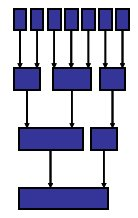
\includegraphics[width=0.8\linewidth,height=\textheight,keepaspectratio]{../../images/AA/aglom.jpg}
\end{center}
\end{column}
\end{columns}
\end{frame}

\begin{frame}{Métodos hierárquicos}
\phantomsection\label{muxe9todos-hieruxe1rquicos-1}
\begin{columns}[T]
\begin{column}{0.75\linewidth}
\begin{itemize}
\tightlist
\item
  \textbf{Divisivos (ou de Partição):} Fazem o caminho oposto aos
  métodos hierárquicos aglomerativos. Neste método, um único grupo de
  objetos é subdividido em dois com a maior distância. Estes subgrupos
  são então particionados sucessivamente até se obter os objetos
  individuais.
\end{itemize}
\end{column}

\begin{column}{0.25\linewidth}
\begin{center}
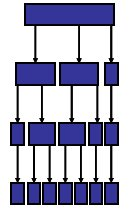
\includegraphics[width=0.8\linewidth,height=\textheight,keepaspectratio]{../../images/AA/part.jpg}
\end{center}
\end{column}
\end{columns}
\end{frame}

\begin{frame}{Métodos de Agrupamento Hierárquicos}
\phantomsection\label{muxe9todos-de-agrupamento-hieruxe1rquicos}
\begin{block}{Agrupamentos hierárquicos aglomerativos}
\phantomsection\label{agrupamentos-hieruxe1rquicos-aglomerativos}
\begin{enumerate}
[a)]
\item
  Considerar inicialmente \(n\) grupos, sendo \(n\) o número de
  indivíduos. A matriz de distâncias \(\boldsymbol{D}_{n \times n}\) é a
  matriz de distâncias entre os elementos originais;
\item
  Selecionar os dois indivíduos mais próximos na matriz
  \(\boldsymbol{D}_{n \times n}\) e formar com eles um grupo;
\item
  Substituir os indivíduos utilizados no passo b) para definir o grupo
  por um novo elemento que represente o grupo construído. A distância
  entre esse novo elemento e os indivíduos restantes são calculadas
  utilizando um dos critérios que serão definidos a seguir;
\item
  Voltar ao passo b) e repetir os passos b) e c) até que tenhamos todos
  os elementos agrupados em um único grupo.
\end{enumerate}
\end{block}
\end{frame}

\begin{frame}{Métodos de Agrupamento Hierárquicos}
\phantomsection\label{muxe9todos-de-agrupamento-hieruxe1rquicos-1}
\begin{block}{Resultado da aplicação do método}
\phantomsection\label{resultado-da-aplicauxe7uxe3o-do-muxe9todo}
\begin{columns}[T]
\begin{column}{0.75\linewidth}
\begin{center}
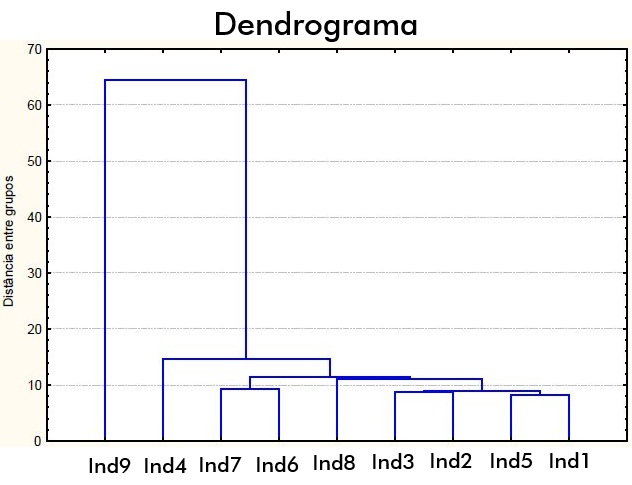
\includegraphics[width=0.8\linewidth,height=\textheight,keepaspectratio]{../../images/AA/dend2.jpg}
\end{center}
\end{column}

\begin{column}{0.25\linewidth}
\begin{itemize}
\item
  Representa uma síntese gráfica do método de agrupamento
\item
  Esse gráfico é de grande utilidade para a classificação, comparação e
  discussão de agrupamentos.
\end{itemize}
\end{column}
\end{columns}
\end{block}
\end{frame}

\begin{frame}{Métodos de Agrupamento Hierárquicos}
\phantomsection\label{muxe9todos-de-agrupamento-hieruxe1rquicos-2}
\begin{block}{Como definir distância entre grupos?}
\phantomsection\label{como-definir-distuxe2ncia-entre-grupos}
\begin{itemize}
\item
  Suponha que temos um grupo \(K\) com \(n_k\) indivíduos e um grupo
  \(L\) com \(n_l\) indivíduos.
\item
  A distância entre os grupos \(K\) e \(L\) pode ser calculada com base
  em um dos cinco métodos seguintes:

  \begin{itemize}
  \tightlist
  \item
    Método do vizinho mais próximo (\emph{single linkage})
  \item
    Método do vizinho mais distante (\emph{complete linkage})
  \item
    Método da distância média (\emph{average linkage})
  \item
    Método do centroide (\emph{Centroid})
  \item
    Método de Ward
  \end{itemize}
\end{itemize}
\end{block}
\end{frame}

\begin{frame}{Métodos de Agrupamento Hierárquicos}
\phantomsection\label{muxe9todos-de-agrupamento-hieruxe1rquicos-3}
\begin{block}{Método do vizinho mais próximo}
\phantomsection\label{muxe9todo-do-vizinho-mais-pruxf3ximo}
Consiste em considerar que a distância entre os dois grupos é a
\textbf{menor distância entre as possíveis combinações de indivíduos}
tomados dos dois grupos considerados, isto é,

\begin{columns}[T]
\begin{column}{0.5\linewidth}
\[\Large d_{(K,L)} =  \underbrace{\min(d_{ij})}_{i \in K, j \in L}\]
\end{column}

\begin{column}{0.5\linewidth}
\begin{center}
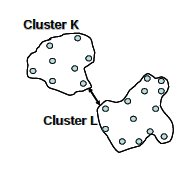
\includegraphics[width=0.8\linewidth,height=\textheight,keepaspectratio]{../../images/AA/mvmp.jpg}
\end{center}
\end{column}
\end{columns}
\end{block}
\end{frame}

\begin{frame}{Métodos de Agrupamento Hierárquicos}
\phantomsection\label{muxe9todos-de-agrupamento-hieruxe1rquicos-4}
\begin{block}{Método do vizinho mais próximo}
\phantomsection\label{muxe9todo-do-vizinho-mais-pruxf3ximo-1}
\textbf{Esquematicamente:}

\begin{center}
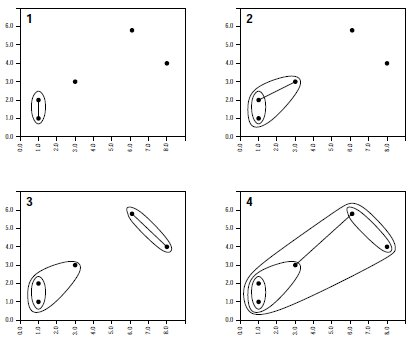
\includegraphics[width=1\linewidth,height=\textheight,keepaspectratio]{../../images/AA/metvmprox.jpg}
\end{center}
\end{block}
\end{frame}

\begin{frame}{Métodos de Agrupamento Hierárquicos}
\phantomsection\label{muxe9todos-de-agrupamento-hieruxe1rquicos-5}
\begin{block}{Método do vizinho mais próximo}
\phantomsection\label{muxe9todo-do-vizinho-mais-pruxf3ximo-2}
\textbf{Esquematicamente:}

\begin{center}
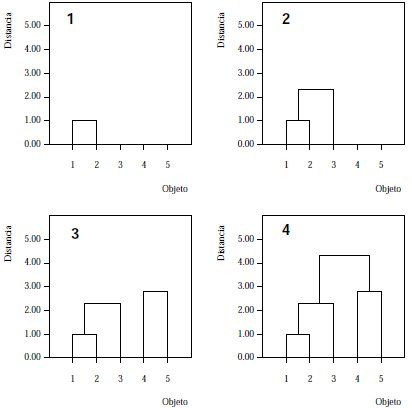
\includegraphics[width=1\linewidth,height=\textheight,keepaspectratio]{../../images/AA/dend_mvmp.jpg}
\end{center}
\end{block}
\end{frame}

\begin{frame}{Métodos de Agrupamento Hierárquicos}
\phantomsection\label{muxe9todos-de-agrupamento-hieruxe1rquicos-6}
\begin{block}{Método do vizinho mais distante}
\phantomsection\label{muxe9todo-do-vizinho-mais-distante}
Consiste em considerar que a distância entre os dois grupos é a
\textbf{maior distância entre as possíveis combinações de indivíduos}
tomados dos dois grupos considerados, isto é,

\begin{columns}[T]
\begin{column}{0.5\linewidth}
\[\Large d_{(K,L)} =  \underbrace{\max(d_{ij})}_{i \in K, j \in L}\]
\end{column}

\begin{column}{0.5\linewidth}
\begin{center}
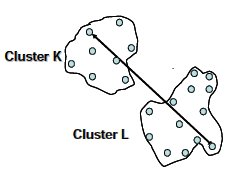
\includegraphics[width=0.8\linewidth,height=\textheight,keepaspectratio]{../../images/AA/mvmd.jpg}
\end{center}
\end{column}
\end{columns}
\end{block}
\end{frame}

\begin{frame}{Métodos de Agrupamento Hierárquicos}
\phantomsection\label{muxe9todos-de-agrupamento-hieruxe1rquicos-7}
\begin{block}{Método da distância média}
\phantomsection\label{muxe9todo-da-distuxe2ncia-muxe9dia}
Consiste em considerar que a distância entre os dois grupos é a
\textbf{média aritmética das distâncias entre as possíveis combinações
de indivíduos} tomados dos dois grupos considerados, isto é,

\begin{columns}[T]
\begin{column}{0.5\linewidth}
\[\Large d_{(K,L)} = \displaystyle{\sum_{i \in K} \sum_{j \in L}} \displaystyle{\frac{d_{ij}}{n_kn_l}}\]
\end{column}

\begin{column}{0.5\linewidth}
\begin{center}
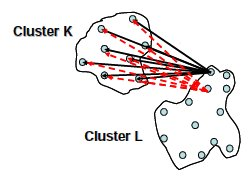
\includegraphics[width=0.8\linewidth,height=\textheight,keepaspectratio]{../../images/AA/mdm.jpg}
\end{center}
\end{column}
\end{columns}
\end{block}
\end{frame}

\begin{frame}{Métodos de Agrupamento Hierárquicos}
\phantomsection\label{muxe9todos-de-agrupamento-hieruxe1rquicos-8}
\begin{block}{Método do centroide}
\phantomsection\label{muxe9todo-do-centroide}
Consiste em considerar que a distância entre os dois grupos é a
\textbf{distância euclidiana ao quadrado entre os centroides} dos dois
grupos. O centroide de um grupo é o ponto médio dos objetos contidos no
grupo, isto é,

\begin{columns}[T]
\begin{column}{0.5\linewidth}
\[\Large d_{(K,L)} = (\bar{K} - \bar{L})^t(\bar{K} - \bar{L})\]

\[\bar{K} = \displaystyle{\frac{\displaystyle{\sum_{i \in K} i}}{n_k}} \hspace{0.2cm} {\rm e} \hspace{0.2cm} 
\bar{L} = \displaystyle{\frac{\displaystyle{\sum_{j \in L} j}}{n_l}}\]
\end{column}

\begin{column}{0.5\linewidth}
\begin{center}
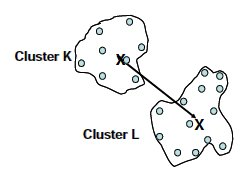
\includegraphics[width=0.8\linewidth,height=\textheight,keepaspectratio]{../../images/AA/mc.jpg}
\end{center}
\end{column}
\end{columns}
\end{block}
\end{frame}

\begin{frame}{Métodos de Agrupamento Hierárquicos}
\phantomsection\label{muxe9todos-de-agrupamento-hieruxe1rquicos-9}
\begin{block}{Método de Ward}
\phantomsection\label{muxe9todo-de-ward}
\begin{itemize}
\tightlist
\item
  Considere a soma de quadrados intra-cluster de um cluster \(A\):
\end{itemize}

\[SQE_A = \displaystyle{\sum_{i = 1}^{n_A}}(x_{i} - \bar{\bf x}_A)^t(x_{i} - \bar{\bf x}_A)\]

\begin{itemize}
\tightlist
\item
  Definimos o acréscimo na soma de quadrados resultante da junção de
  dois clusters \(A\) e \(B\) em um cluster \(AB\) por:
\end{itemize}

\[I_{AB} = SQE_{AB} - (SQE_A + SQE_B)\]
\end{block}
\end{frame}

\begin{frame}{Métodos de Agrupamento Hierárquicos}
\phantomsection\label{muxe9todos-de-agrupamento-hieruxe1rquicos-10}
\begin{block}{Método de Ward}
\phantomsection\label{muxe9todo-de-ward-1}
\begin{itemize}
\item
  A união entre clusters \(A\) e \(B\) que proporcionarem menor
  acréscimo na \(SQE\) é executada.
\item
  Para usar o método de Ward, as variáveis devem ser
  \textbf{quantitativas}.
\end{itemize}
\end{block}
\end{frame}

\begin{frame}{Métodos de Agrupamento Hierárquicos}
\phantomsection\label{muxe9todos-de-agrupamento-hieruxe1rquicos-11}
\begin{block}{Exemplo}
\phantomsection\label{exemplo}
\begin{columns}[T]
\begin{column}{0.7\linewidth}
A fim de exemplificar a aplicação dos métodos de agrupamento, considere
os dados da Tabela ao lado. Os sete casos são considerados as
observações de cada indivíduo para as variáveis \(X_1\) e \(X_2\).
\end{column}

\begin{column}{0.3\linewidth}
\begin{longtable}[]{@{}rrr@{}}
\toprule\noalign{}
Caso & \(X_1\) & \(X_2\) \\
\midrule\noalign{}
\endhead
1 & 1 & 1 \\
2 & 2 & 1 \\
3 & 3 & 2 \\
4 & 2 & 4,5 \\
5 & 1 & 5 \\
6 & 3 & 7 \\
7 & 6 & 5 \\
\bottomrule\noalign{}
\end{longtable}
\end{column}
\end{columns}
\end{block}
\end{frame}

\begin{frame}{Métodos de Agrupamento Hierárquicos}
\phantomsection\label{muxe9todos-de-agrupamento-hieruxe1rquicos-12}
\begin{block}{Exemplo}
\phantomsection\label{exemplo-1}
\textbf{Representação dos casos no plano}

\begin{center}
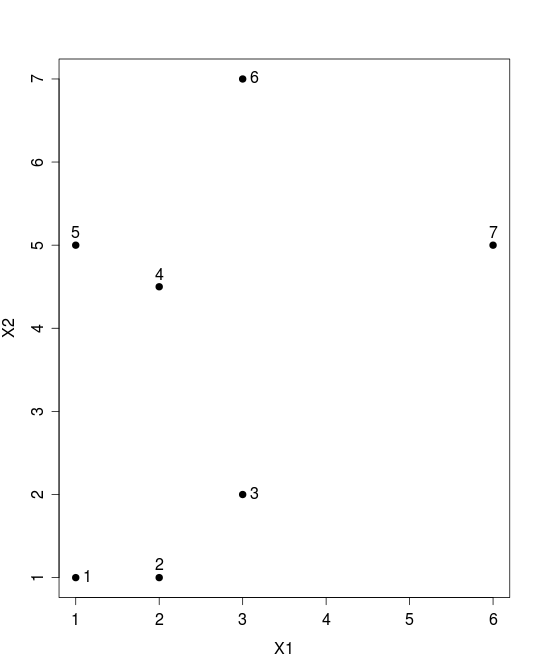
\includegraphics[width=0.8\linewidth,height=\textheight,keepaspectratio]{../../images/AA/plano.jpg}
\end{center}
\end{block}
\end{frame}

\begin{frame}{Métodos de Agrupamento Hierárquicos}
\phantomsection\label{muxe9todos-de-agrupamento-hieruxe1rquicos-13}
\begin{block}{Exemplo}
\phantomsection\label{exemplo-2}
\textbf{Matriz de distâncias}

\[D_0 = \left[ \begin{matrix}
&1 & 2&3&4&5&6&7\\ 
1& 0,000 & 1,000 & 2,236 & 3,640 & 4,000 & 6,325 & 6,403 \\
2&  & 0,000 & 1,414 & 3,500 & 4,123 & 6,083 & 5,657 \\
3&  &  & 0,000 & 2,693 & 3,606 & 5,000 & 4,243 \\
4&  &  &  & 0,000 & 1,118 & 2,693 & 4,031 \\
5& &  &  &  & 0,000 & 2,828 & 5,000 \\
6&  &  &  &  &  & 0,000 & 3,606 \\
7&  &  &  &  &  &  & 0,000
                    \end{matrix} \right]\]
\end{block}
\end{frame}

\begin{frame}{Métodos de Agrupamento Hierárquicos}
\phantomsection\label{muxe9todos-de-agrupamento-hieruxe1rquicos-14}
\begin{block}{Exemplo}
\phantomsection\label{exemplo-3}
\textbf{Matriz de distâncias}

\[D_0 = \left[ \begin{matrix}
&1 & 2&3&4&5&6&7\\ 
1& 0,000 & \textbf{1,000} & 2,236 & 3,640 & 4,000 & 6,325 & 6,403 \\
2&  & 0,000 & 1,414 & 3,500 & 4,123 & 6,083 & 5,657 \\
3&  &  & 0,000 & 2,693 & 3,606 & 5,000 & 4,243 \\
4&  &  &  & 0,000 & 1,118 & 2,693 & 4,031 \\
5& &  &  &  & 0,000 & 2,828 & 5,000 \\
6&  &  &  &  &  & 0,000 & 3,606 \\
7&  &  &  &  &  &  & 0,000
                    \end{matrix} \right]\]

\[\scriptsize d_{12} = \sqrt{\displaystyle{(X_{11} - X_{21})^2 + (X_{12} - X_{22})^2}} = 
\sqrt{\displaystyle{(1 - 1)^2 + (2 - 1)^2}} = \sqrt{1} = 1\]
\end{block}
\end{frame}

\begin{frame}{Métodos de Agrupamento Hierárquicos}
\phantomsection\label{muxe9todos-de-agrupamento-hieruxe1rquicos-15}
\begin{block}{Exemplo}
\phantomsection\label{exemplo-4}
\textbf{Passo 1: juntar os casos 1 e 2}

\begin{itemize}
\item
  Redefinir a matriz de distâncias considerando os casos mais parecidos
  como se fossem um único grupo.
\item
  \textbf{Aqui os métodos se diferenciam!}
\item
  \textbf{Método do vizinho mais próximo}
\end{itemize}
\end{block}
\end{frame}

\begin{frame}{Métodos de Agrupamento Hierárquicos}
\phantomsection\label{muxe9todos-de-agrupamento-hieruxe1rquicos-16}
\begin{block}{Exemplo}
\phantomsection\label{exemplo-5}
\textbf{Construção da nova matriz de distâncias}

\[
\begin{aligned}
d_{((1,2)3)} &=  \min(d_{13};d_{23}) = \min(2,236; 1,414) = 1,414 \\[6pt]
d_{((1,2)4)} &=  \min(d_{14};d_{24}) = \min(3,640; 3,500) = 3,500 \\[6pt]
d_{((1,2)5)} &=  \min(d_{15};d_{25}) = \min(4,000; 4,123) = 4,000 \\[6pt]
d_{((1,2)6)} &=  \min(d_{16};d_{26}) = \min(6,325; 6,083) = 6,083 \\[6pt]
d_{((1,2)7)} &=  \min(d_{17};d_{27}) = \min(6,403; 5,657) = 5,657
\end{aligned}
\]
\end{block}
\end{frame}

\begin{frame}{Métodos de Agrupamento Hierárquicos}
\phantomsection\label{muxe9todos-de-agrupamento-hieruxe1rquicos-17}
\begin{block}{Exemplo}
\phantomsection\label{exemplo-6}
\textbf{Matriz de distâncias}

\[D_1 = \left[ \begin{matrix}
&(1,2)&3&4&5&6&7\\ 
(1,2)& 0,000 & 1,414 & 3,500 & 4,000 & 6,083 & 5,657 \\
3  &  & 0,000 & 2,693 & 3,606 & 5,000 & 4,243 \\
4  &  &  & 0,000 & 1,118 & 2,693 & 4,031 \\
5 &  &  &  & 0,000 & 2,828 & 5,000 \\
6  &  &  &  &  & 0,000 & 3,606 \\
7  &  &  &  &  &  & 0,000
                    \end{matrix} \right]\]
\end{block}
\end{frame}

\begin{frame}{Métodos de Agrupamento Hierárquicos}
\phantomsection\label{muxe9todos-de-agrupamento-hieruxe1rquicos-18}
\begin{block}{Exemplo}
\phantomsection\label{exemplo-7}
\textbf{Matriz de distâncias}

\[D_1 = \left[ \begin{matrix}
&(1,2)&3&4&5&6&7\\ 
(1,2)& 0,000 & 1,414 & 3,500 & 4,000 & 6,083 & 5,657 \\
3  &  & 0,000 & 2,693 & 3,606 & 5,000 & 4,243 \\
4  &  &  & 0,000 & \textbf{1,118} & 2,693 & 4,031 \\
5 &  &  &  & 0,000 & 2,828 & 5,000 \\
6  &  &  &  &  & 0,000 & 3,606 \\
7  &  &  &  &  &  & 0,000
                    \end{matrix} \right]\]
\end{block}
\end{frame}

\begin{frame}{Métodos de Agrupamento Hierárquicos}
\phantomsection\label{muxe9todos-de-agrupamento-hieruxe1rquicos-19}
\begin{block}{Exemplo}
\phantomsection\label{exemplo-8}
\textbf{Passo 2: juntar os casos 4 e 5}

\textbf{Redefinir a matriz de distâncias considerando os casos mais
parecidos como se fossem um único grupo.}

\[
\begin{aligned}
d_{((4,5)(1,2))} &=  \min(d_{14};d_{24};d_{15};d_{25}) = \min(3,640; 3,500; 4,000; 4,123) = 3,500 \\ &= 
\min(d_{(1,2)4};d_{(1,2)5}) = \min(3,500;4,000) \\
d_{((4,5)3)} &=  \min(d_{34};d_{35}) = \min(2,693; 3,606) = 2,693 \\
d_{((4,5)6)} &=  \min(d_{46};d_{56}) = \min(2,693; 2,828) = 2,693 \\
d_{((4,5)7)} &=  \min(d_{47};d_{57}) = \min(4,031; 5,000) = 4,031 
\end{aligned}
\]
\end{block}
\end{frame}

\begin{frame}{Métodos de Agrupamento Hierárquicos}
\phantomsection\label{muxe9todos-de-agrupamento-hieruxe1rquicos-20}
\begin{block}{Exemplo}
\phantomsection\label{exemplo-9}
\textbf{Matriz de distâncias}

\[D_2 = \left[ \begin{matrix}
&(1,2)&3&(4,5)&6&7\\ 
(1,2)& 0,000 & 1,414 & 3,500 &  6,083 & 5,657 \\
3  &  & 0,000 & 2,693 & 5,000 & 4,243 \\
(4,5)  &  &  & 0,000 &  2,693 & 4,031 \\
6  &  &    &  & 0,000 & 3,606 \\
7  &  &    &  &  & 0,000
                    \end{matrix} \right]\]
\end{block}
\end{frame}

\begin{frame}{Métodos de Agrupamento Hierárquicos}
\phantomsection\label{muxe9todos-de-agrupamento-hieruxe1rquicos-21}
\begin{block}{Exemplo}
\phantomsection\label{exemplo-10}
\textbf{Matriz de distâncias}

\[D_2 = \left[ \begin{matrix}
&(1,2)&3&(4,5)&6&7\\ 
(1,2)& 0,000 & \textbf{1,414} & 3,500 &  6,083 & 5,657 \\
3  &  & 0,000 & 2,693 & 5,000 & 4,243 \\
(4,5)  &  &  & 0,000 &  2,693 & 4,031 \\
6  &  &    &  & 0,000 & 3,606 \\
7  &  &    &  &  & 0,000
                    \end{matrix} \right]\]
\end{block}
\end{frame}

\begin{frame}{Métodos de Agrupamento Hierárquicos}
\phantomsection\label{muxe9todos-de-agrupamento-hieruxe1rquicos-22}
\begin{block}{Exemplo}
\phantomsection\label{exemplo-11}
\textbf{Passo 3: juntar o grupo \((1,2)\) como caso 3}

\textbf{Redefinir a matriz de distâncias considerando os casos mais
parecidos como se fossem um único grupo.}

\[ \small
\begin{aligned}
d_{(((1,2,3)(4,5))} &=  \min(d_{14};d_{24};d_{34};d_{15};d_{25};d_{35}) \\ &= \min(3,640; 3,500; 2,693; 4,000; 4,123; 3,606) = 2,693 \\ &= 
\min(d_{(1,2)(4,5)};d_{(4,5)3}) = \min(3,500;2,693) \\
d_{((1,2,3)6)} &= \min(d_{16};d_{26};d_{36}) =  \min(6,325; 6,083; 5,000) = 5,000 \\ &=  \min(d_{((1,2)6)};d_{36}) = \min(6,083;5,000) \\
d_{((1,2,3)7)} &= \min(d_{17};d_{27};d_{37}) =  \min(6,403; 5,657; 4,243) = 4,243 \\ &=  \min(d_{((1,2)7)};d_{37}) = \min(5,657;4,243) \\ 
\end{aligned}
\]
\end{block}
\end{frame}

\begin{frame}{Métodos de Agrupamento Hierárquicos}
\phantomsection\label{muxe9todos-de-agrupamento-hieruxe1rquicos-23}
\begin{block}{Exemplo}
\phantomsection\label{exemplo-12}
\textbf{Matriz de distâncias}

\[D_3 = \left[ \begin{matrix}
&(1,2,3) &(4,5)&6&7\\ 
(1,2,3)& 0,000 & 2,693 & 5,000 & 4,243 \\
(4,5)    &  & 0,000 &  2,693 & 4,031 \\
6  &     &  & 0,000 & 3,606 \\
7  &      &  &  & 0,000
                    \end{matrix} \right]\]
\end{block}
\end{frame}

\begin{frame}{Métodos de Agrupamento Hierárquicos}
\phantomsection\label{muxe9todos-de-agrupamento-hieruxe1rquicos-24}
\begin{block}{Exemplo}
\phantomsection\label{exemplo-13}
\textbf{Matriz de distâncias}

\[D_3 = \left[ \begin{matrix}
&(1,2,3) &(4,5)&6&7\\ 
(1,2,3)& 0,000 & \textbf{2,693} & 5,000 & 4,243 \\
(4,5)    &  & 0,000 &  \textbf{2,693} & 4,031 \\
6  &     &  & 0,000 & 3,606 \\
7  &      &  &  & 0,000
                    \end{matrix} \right]\]
\end{block}
\end{frame}

\begin{frame}{Métodos de Agrupamento Hierárquicos}
\phantomsection\label{muxe9todos-de-agrupamento-hieruxe1rquicos-25}
\begin{block}{Exemplo}
\phantomsection\label{exemplo-14}
\textbf{Passo 4: juntar o grupo \((4,5)\) como caso 6}

\textbf{Redefinir a matriz de distâncias considerando os casos mais
parecidos como se fossem um único grupo.}

\[ \small
\begin{aligned}
d_{(((4,5,6)(1,2,3))} &=  \min(d_{14};d_{24};d_{34};d_{15};d_{25};d_{35};d_{16};d_{26};d_{36}) \\ 
&= \min(3,640; 3,500; 2,693; 4,000; 4,123; 3,606; 6,325; 6,083; 5,000) = 2,693 \\ &= 
\min(d_{(1,2,3)(4,5)};d_{(1,2,3)6}) = \min(2,693; 5,000) \\
d_{((4,5,6)7)} &= \min(d_{47};d_{57};d_{67}) =  \min(4,031; 5,000; 3,606) = 3,606 \\ &=  \min(d_{((4,5)7)};d_{67}) = \min(4,031;3,606) \\ 
\end{aligned}
\]
\end{block}
\end{frame}

\begin{frame}{Métodos de Agrupamento Hierárquicos}
\phantomsection\label{muxe9todos-de-agrupamento-hieruxe1rquicos-26}
\begin{block}{Exemplo}
\phantomsection\label{exemplo-15}
\textbf{Matriz de distâncias}

\[D_4 = \left[ \begin{matrix}
&(1,2,3) &(4,5,6) &7\\ 
(1,2,3)& 0,000 & 2,693 &  4,243 \\
(4,5,6)    &  & 0,000 &  3,606 \\
7  &       &  & 0,000
                    \end{matrix} \right]\]
\end{block}
\end{frame}

\begin{frame}{Métodos de Agrupamento Hierárquicos}
\phantomsection\label{muxe9todos-de-agrupamento-hieruxe1rquicos-27}
\begin{block}{Exemplo}
\phantomsection\label{exemplo-16}
\textbf{Matriz de distâncias}

\[D_4 = \left[ \begin{matrix}
&(1,2,3) &(4,5,6) &7\\ 
(1,2,3)& 0,000 & \textbf{2,693} &  4,243 \\
(4,5,6)    &  & 0,000 &  3,606 \\
7  &       &  & 0,000
                    \end{matrix} \right]\]
\end{block}
\end{frame}

\begin{frame}{Métodos de Agrupamento Hierárquicos}
\phantomsection\label{muxe9todos-de-agrupamento-hieruxe1rquicos-28}
\begin{block}{Exemplo}
\phantomsection\label{exemplo-17}
\textbf{Passo 5: juntar o grupo \((1,2,3)\) com o grupo \((4,5,6)\)}

\textbf{Redefinir a matriz de distâncias considerando os casos mais
parecidos como se fossem um único grupo.}

\[
\begin{aligned}
d_{((1,2,3,4,5,6)7)} &=  \min(d_{17};d_{27};d_{37};d_{47};d_{57};d_{67}) \\ 
&= \min(6,403; 5,657; 4,243; 4,031; 5,000; 3,606) = 3,606 \\ &= 
\min(d_{(1,2,3)7};d_{(4,5,6)7}) = \min(4,243; 3,606) \\
\end{aligned}
\]
\end{block}
\end{frame}

\begin{frame}{Métodos de Agrupamento Hierárquicos}
\phantomsection\label{muxe9todos-de-agrupamento-hieruxe1rquicos-29}
\begin{block}{Exemplo}
\phantomsection\label{exemplo-18}
\textbf{Matriz de distâncias}

\[D_5 = \left[ \begin{matrix}
&(1,2,3,4,5,6) & 7\\ 
(1,2,3,4,5,6 )& 0,000 & 3,606 \\
7         &  & 0,000
                    \end{matrix} \right]\]
\end{block}
\end{frame}

\begin{frame}{Métodos de Agrupamento Hierárquicos}
\phantomsection\label{muxe9todos-de-agrupamento-hieruxe1rquicos-30}
\begin{block}{Exemplo}
\phantomsection\label{exemplo-19}
\textbf{Matriz de distâncias}

\[D_5 = \left[ \begin{matrix}
&(1,2,3,4,5,6) & 7\\ 
(1,2,3,4,5,6 )& 0,000 & \textbf{3,606} \\
7         &  & 0,000
                    \end{matrix} \right]\]
\end{block}
\end{frame}

\begin{frame}{Métodos de Agrupamento Hierárquicos}
\phantomsection\label{muxe9todos-de-agrupamento-hieruxe1rquicos-31}
\begin{block}{Exemplo}
\phantomsection\label{exemplo-20}
\textbf{Resumo do método de agrupamento}

\begin{longtable}[]{@{}rrlr@{}}
\toprule\noalign{}
Passo & Nº de grupos & Grupos & Distância \\
\midrule\noalign{}
\endhead
1 & 7 & 1, 2, 3, 4, 5, 6, 7 & 0,000 \\
2 & 6 & (1,2), 3, 4, 5, 6, 7 & 1,000 \\
3 & 5 & (1,2), 3, (4,5), 6, 7 & 1,118 \\
4 & 4 & (1,2,3), (4,5), 6, 7 & 1,414 \\
5 & 3 & (1,2,3), (4,5,6), 7 & 2,693 \\
6 & 2 & (1,2,3,4,5,6), 7 & 2,693 \\
7 & 1 & (1,2,3,4,5,6,7) & 3,606 \\
\bottomrule\noalign{}
\end{longtable}
\end{block}
\end{frame}

\begin{frame}{Métodos de Agrupamento Hierárquicos}
\phantomsection\label{muxe9todos-de-agrupamento-hieruxe1rquicos-32}
\begin{block}{Exemplo}
\phantomsection\label{exemplo-21}
\begin{center}
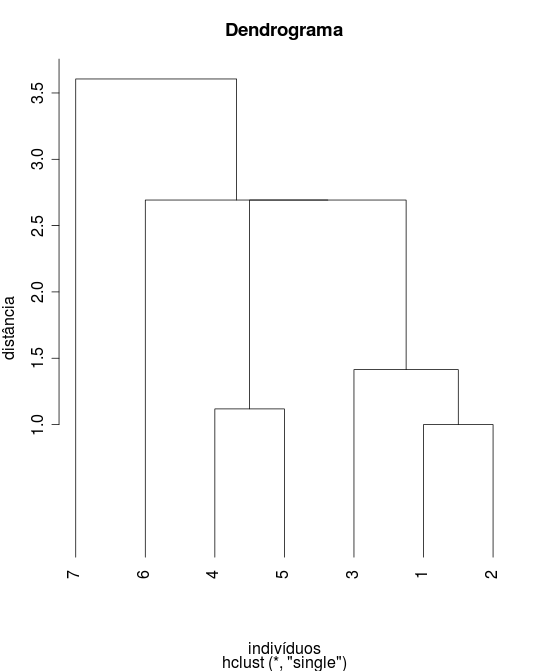
\includegraphics[width=1\linewidth,height=\textheight,keepaspectratio]{../../images/AA/dend3.jpg}
\end{center}
\end{block}
\end{frame}

\begin{frame}{Métodos de Agrupamento Hierárquicos}
\phantomsection\label{muxe9todos-de-agrupamento-hieruxe1rquicos-33}
\begin{block}{Determinação do número de grupos}
\phantomsection\label{determinauxe7uxe3o-do-nuxfamero-de-grupos}
\begin{itemize}
\item
  O dendrograma permite ao pesquisador consultar a distância em que os
  clusters foram combinados para formar um novo cluster.
\item
  Clusters que são semelhantes entre si são combinados a baixas
  distâncias, enquanto grupos que são mais dissimilares são combinados
  em altas distâncias.
\item
  A diferença de distâncias define como os clusters próximos são um do
  outro.
\end{itemize}
\end{block}
\end{frame}

\begin{frame}{Métodos de Agrupamento Hierárquicos}
\phantomsection\label{muxe9todos-de-agrupamento-hieruxe1rquicos-34}
\begin{block}{Determinação do número de grupos}
\phantomsection\label{determinauxe7uxe3o-do-nuxfamero-de-grupos-1}
\begin{itemize}
\item
  Uma partição dos dados em um número especificado de grupos pode ser
  obtida ``cortando'' o dendograma a uma distância apropriada.
\item
  Se traçarmos uma linha horizontal no dendograma a uma determinada
  distância, então o número \(k\) das linhas verticais cortadas por essa
  linha horizontal identificará uma solução \(k\)-cluster.
\item
  A intersecção da linha horizontal e uma dessas linhas verticais
  representa um cluster, e os itens localizados no final de todos os
  ramos abaixo interseção constituem os membros do cluster.
\end{itemize}
\end{block}
\end{frame}

\begin{frame}{Métodos de Agrupamento Hierárquicos}
\phantomsection\label{muxe9todos-de-agrupamento-hieruxe1rquicos-35}
\begin{block}{Determinação do número de grupos}
\phantomsection\label{determinauxe7uxe3o-do-nuxfamero-de-grupos-2}
\begin{center}
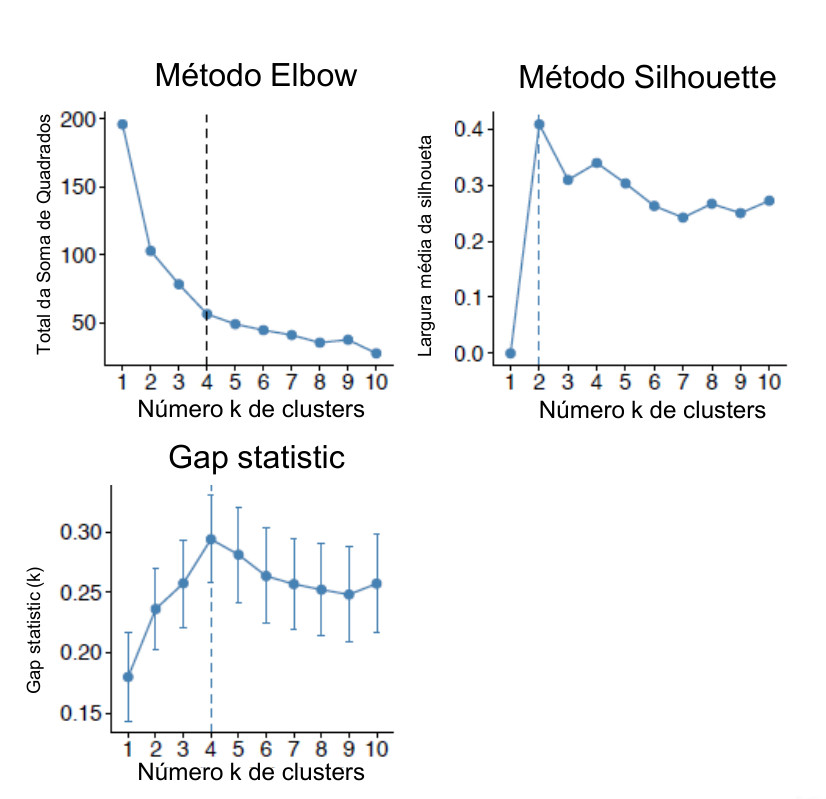
\includegraphics[width=1\linewidth,height=\textheight,keepaspectratio]{../../images/AA/num_grupos.jpg}
\end{center}
\end{block}
\end{frame}

\begin{frame}{Métodos hierárquicos: comentários finais}
\phantomsection\label{muxe9todos-hieruxe1rquicos-comentuxe1rios-finais}
\begin{itemize}
\tightlist
\item
  Fontes de erros e de variação não são formalmente considerados nos
  procedimentos hierárquicos: Significa que esses métodos são sensíveis
  a outliers ou pontos de perturbação
\end{itemize}

\pause

\begin{itemize}
\tightlist
\item
  Deve-se sempre verificar a sensibilidade da configuração dos grupos:
  Os métodos não permitem a realocação de objetos que possam ter sido
  agrupados incorretamente nos estágios iniciais
\end{itemize}

\pause

\begin{itemize}
\tightlist
\item
  É recomendado tentar vários métodos de agrupamento e de atribuição de
  distâncias (similaridades)
\end{itemize}

\pause

\begin{itemize}
\tightlist
\item
  Empates na matriz de distâncias podem produzir múltiplas soluções ao
  problema de agrupamento hierárquico
\end{itemize}
\end{frame}

\begin{frame}{Métodos hierárquicos: comentários finais}
\phantomsection\label{muxe9todos-hieruxe1rquicos-comentuxe1rios-finais-1}
\begin{itemize}
\tightlist
\item
  A maioria dos métodos produz clusters esféricos ou elípticos
\end{itemize}

\pause

\begin{itemize}
\tightlist
\item
  O método de \textbf{ligação simples} é um dos poucos métodos que pode
  delinear cluster não-elípticos

  \begin{itemize}
  \tightlist
  \item
    Tem a capacidade de gerar estruturas geométricas diferentes
  \item
    Entretanto, ele é incapaz de perceber grupos pouco separados
  \end{itemize}
\end{itemize}

\pause

\begin{itemize}
\tightlist
\item
  Os clusters formados pelo método de ligação simples não serão
  modificados por qualquer atribuição de distância (similaridade) que dá
  as mesmas ordenações relativas
\end{itemize}
\end{frame}

\begin{frame}{Métodos hierárquicos: comentários finais}
\phantomsection\label{muxe9todos-hieruxe1rquicos-comentuxe1rios-finais-2}
\begin{itemize}
\tightlist
\item
  O método de \textbf{ligação completa} tende a produzir conglomerados
  de aproximadamente mesmo diâmetro

  \begin{itemize}
  \tightlist
  \item
    Tem a tendência de isolar os valores discrepantes nos estágios
    iniciais do agrupamento
  \end{itemize}
\end{itemize}

\pause

\begin{itemize}
\tightlist
\item
  O método da \textbf{média das distâncias} tende a produzir
  conglomerados de aproximadamente mesma variância interna

  \begin{itemize}
  \tightlist
  \item
    Em geral, produz melhores partições que os métodos de ligação
    simples e completa
  \end{itemize}
\end{itemize}
\end{frame}

\begin{frame}{Métodos hierárquicos: comentários finais}
\phantomsection\label{muxe9todos-hieruxe1rquicos-comentuxe1rios-finais-3}
\begin{itemize}
\tightlist
\item
  Os métodos de ligação simples, completa e da média podem ser
  utilizados tanto para \textbf{variáveis quantitativas} quanto para
  \textbf{variáveis qualitativas}
\end{itemize}

\pause

\begin{itemize}
\tightlist
\item
  Os métodos do centróide e de Ward são apropriados apenas para
  \textbf{variáveis quantitativas}
\end{itemize}

\pause

\begin{itemize}
\tightlist
\item
  O \textbf{método de Ward} tende a produzir grupos com aproximadamente
  o mesmo número de elementos
\end{itemize}

\pause

\begin{itemize}
\tightlist
\item
  Espera-se sempre que haja uma certa consistência entre as soluções
  obtidas por métodos diferentes: pode não ocorrer a igualdade das
  soluções apresentadas pelos vários métodos
\end{itemize}
\end{frame}

\begin{frame}{Validação dos agrupamentos}
\phantomsection\label{validauxe7uxe3o-dos-agrupamentos}
\begin{itemize}
\tightlist
\item
  MANOVA
\end{itemize}

\pause

\begin{itemize}
\tightlist
\item
  Análise Discriminante
\end{itemize}

\pause

\begin{itemize}
\tightlist
\item
  Correlação Cofenética
\end{itemize}

\pause

\begin{itemize}
\tightlist
\item
  Gráfico da Silhueta
\end{itemize}
\end{frame}

\begin{frame}{Validação dos agrupamentos}
\phantomsection\label{validauxe7uxe3o-dos-agrupamentos-1}
\begin{block}{Correlação Cofenética}
\phantomsection\label{correlauxe7uxe3o-cofenuxe9tica}
\begin{itemize}
\item
  Medida de validação usada nos métodos hierárquicos principalmente
\item
  \textbf{Idéia:} realizar uma comparação das distâncias observadas e
  preditas (via a formação de agrupamentos) entre os objetos
\end{itemize}
\end{block}
\end{frame}

\begin{frame}{Validação dos agrupamentos}
\phantomsection\label{validauxe7uxe3o-dos-agrupamentos-2}
\begin{center}
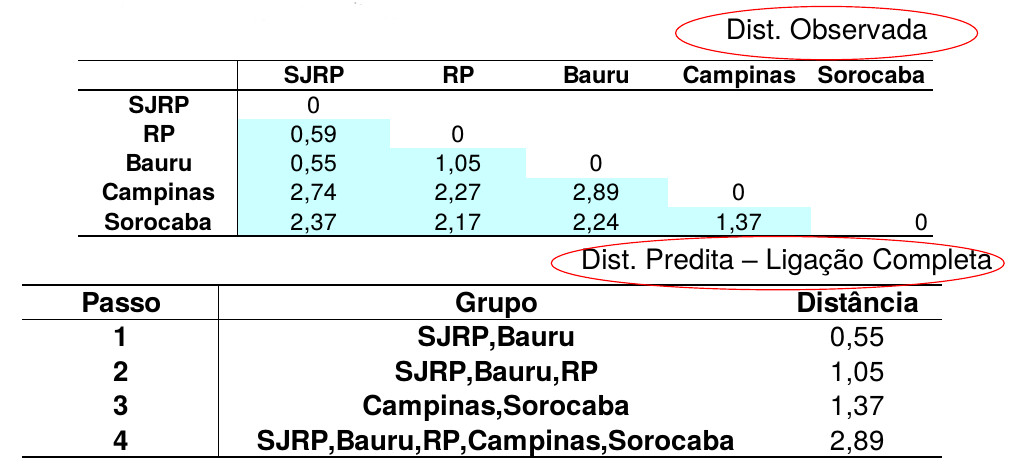
\includegraphics[width=1\linewidth,height=\textheight,keepaspectratio]{../../images/AA/ccofenetica01.jpg}
\end{center}
\end{frame}

\begin{frame}{Validação dos agrupamentos}
\phantomsection\label{validauxe7uxe3o-dos-agrupamentos-3}
\begin{center}
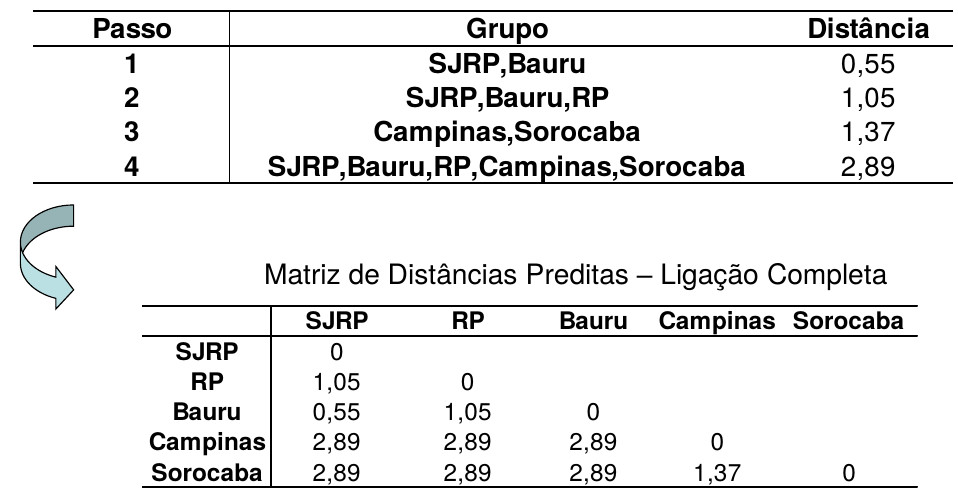
\includegraphics[width=1\linewidth,height=\textheight,keepaspectratio]{../../images/AA/ccofenetica02.jpg}
\end{center}
\end{frame}

\begin{frame}{Validação dos agrupamentos}
\phantomsection\label{validauxe7uxe3o-dos-agrupamentos-4}
\begin{center}
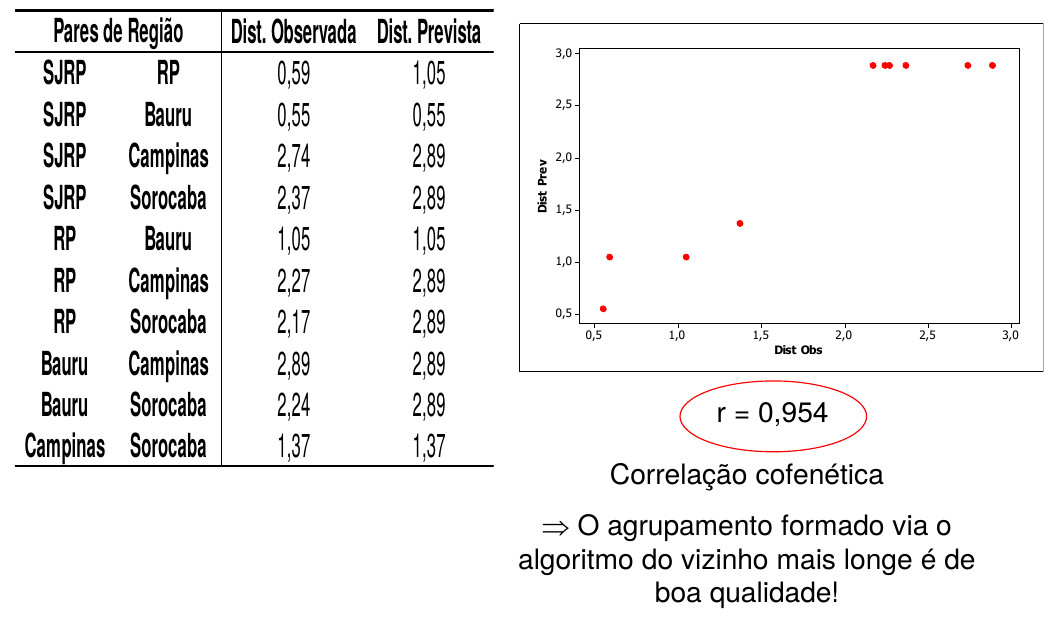
\includegraphics[width=1\linewidth,height=\textheight,keepaspectratio]{../../images/AA/ccofenetica03.jpg}
\end{center}
\end{frame}

\begin{frame}{Validação dos agrupamentos}
\phantomsection\label{validauxe7uxe3o-dos-agrupamentos-5}
\begin{block}{Correlação Cofenética}
\phantomsection\label{correlauxe7uxe3o-cofenuxe9tica-1}
\begin{itemize}
\item
  Em um bom agrupamento, espera-se que as distâncias previstas respeitem
  a ordem determinada pelas distâncias observadas.
\item
  Para avaliar a ocorrência desse comportamento, define-se a correlação
  cofenética como sendo a correlação entre as distâncias efetivamente
  observadas e as previstas.
\end{itemize}
\end{block}
\end{frame}

\begin{frame}{Validação dos agrupamentos}
\phantomsection\label{validauxe7uxe3o-dos-agrupamentos-6}
\begin{block}{Gráfico da Silhueta}
\phantomsection\label{gruxe1fico-da-silhueta}
\begin{itemize}
\item
  A análise (gráfico) da silhueta é um método utilizado para
  interpretação e validação de uma análise de clusters.
\item
  Consiste no cálculo e representação gráfica de uma medida de quão bem
  cada elemento está alocado ao respectivo cluster.
\item
  Tomando a média dessas medidas em um particular cluster, tem-se uma
  medida de coesão do cluster;
\item
  Tomando-se a média dessas medidas em toda a amostra, tem-se uma medida
  de consistência dos agrupamentos formados.
\end{itemize}
\end{block}
\end{frame}

\begin{frame}{Validação dos agrupamentos}
\phantomsection\label{validauxe7uxe3o-dos-agrupamentos-7}
\begin{block}{Gráfico da Silhueta}
\phantomsection\label{gruxe1fico-da-silhueta-1}
\begin{itemize}
\item
  \(a_{(i)}\) = distância média do objeto \(i\) para os elementos de seu
  próprio grupo
\item
  \(b_{(i)}\) = distância média do objeto \(i\) para os elementos do
  grupo mais próximo
\end{itemize}

\[s_{(i)} = \displaystyle{\dfrac{b_{(i)} - a_{(i)}}{\max(b_{(i)},a_{(i)})}}, \,\,\, i = 1, \cdots, n\]

\begin{itemize}
\tightlist
\item
  Por definição, \(-1 \leqslant s_{(i)} \leqslant 1\).
\end{itemize}
\end{block}
\end{frame}

\begin{frame}{Validação dos agrupamentos}
\phantomsection\label{validauxe7uxe3o-dos-agrupamentos-8}
\begin{block}{Gráfico da Silhueta}
\phantomsection\label{gruxe1fico-da-silhueta-2}
\begin{itemize}
\item
  Se \(a_{(i)} <<< b_{(i)}, s_{(i)} \approx 1\), indicando que \(i\) é
  muito menos dissimilar dos elementos de seu grupo do que dos elementos
  dos outros grupos (\(i\) está bem alocado);
\item
  Se \(a_{(i)} >>> b_{(i)}, s_{(i)} \approx −1\), indicando que \(i\) é
  muito mais dissimilar dos elementos de seu grupo do que dos elementos
  do grupo vizinho (\(i\) está mal alocado);
\item
  Se \(a_{(i)} \approx b_{(i)}, s_{(i)} \approx 0\), indicando que \(i\)
  está na fronteira de seu grupo e do grupo vizinho.
\end{itemize}
\end{block}
\end{frame}

\begin{frame}{Validação dos agrupamentos}
\phantomsection\label{validauxe7uxe3o-dos-agrupamentos-9}
\begin{block}{Gráfico da Silhueta}
\phantomsection\label{gruxe1fico-da-silhueta-3}
\begin{longtable}[]{@{}
  >{\raggedright\arraybackslash}p{(\linewidth - 2\tabcolsep) * \real{0.4043}}
  >{\raggedright\arraybackslash}p{(\linewidth - 2\tabcolsep) * \real{0.5957}}@{}}
\toprule\noalign{}
\begin{minipage}[b]{\linewidth}\raggedright
\textbf{Silhueta Média}
\end{minipage} & \begin{minipage}[b]{\linewidth}\raggedright
\textbf{Interpretação Sugerida}
\end{minipage} \\
\midrule\noalign{}
\endhead
\(0{,}71 - 1{,}00\) & Grupos encontrados possuem estrutura muito
robusta \\
\(0{,}51 - 0{,}70\) & Grupos razoavelmente unidos \\
\(0{,}26 - 0{,}50\) & A estrutura encontrada é fraca, tente outros
métodos de agrupamento \\
\(\leqslant 0{,}25\) & Nenhuma estrutura encontrada \\
\bottomrule\noalign{}
\end{longtable}
\end{block}
\end{frame}

\begin{frame}{Métodos de agrupamento não-hierárquicos - MANH}
\phantomsection\label{muxe9todos-de-agrupamento-nuxe3o-hieruxe1rquicos---manh}
\begin{itemize}
\tightlist
\item
  Os MANH não se baseiam em sucessivas aglomerações (ou partições) dos
  elementos com base numa matiz de distâncias;
\end{itemize}

\pause

\begin{itemize}
\tightlist
\item
  Nos MANH tem-se a possibilidade de realocar indivíduos entre clusters
  ao longo do processo, diferentemente do que ocorre nos métodos
  hierárquicos;
\end{itemize}

\pause

\begin{itemize}
\tightlist
\item
  Há diferentes técnicas não hierárquicas de agrupamento, dentre as
  quais aquelas baseadas em partições amostrais (particularmente o
  algoritmo k-means) são as mais populares.
\end{itemize}
\end{frame}

\begin{frame}{Método k-médias (\emph{k-means})}
\phantomsection\label{muxe9todo-k-muxe9dias-k-means}
\begin{enumerate}
[a)]
\tightlist
\item
  Selecionar aleatoriamente \(k\) indivíduos como centroides iniciais
  (ou escolha os centroides iniciais de alguma forma);
\end{enumerate}

\pause

\begin{enumerate}
[a)]
\setcounter{enumi}{1}
\tightlist
\item
  Calcular as distâncias entre cada indivíduo e o centro de cada um dos
  \(k\) grupos e classificar o indivíduo no grupo mais próximo.
\end{enumerate}

\pause

\begin{enumerate}
[a)]
\setcounter{enumi}{2}
\tightlist
\item
  Calcule o centroide de cada grupo;
\end{enumerate}

\pause

\begin{enumerate}
[a)]
\setcounter{enumi}{3}
\tightlist
\item
  Repita os passos \(b)\) e \(c)\) até que os centroides não apresentem
  mais mudanças.
\end{enumerate}
\end{frame}

\begin{frame}{Método k-médias (\emph{k-means})}
\phantomsection\label{muxe9todo-k-muxe9dias-k-means-1}
\begin{block}{Esquematicamente}
\phantomsection\label{esquematicamente}
\begin{center}
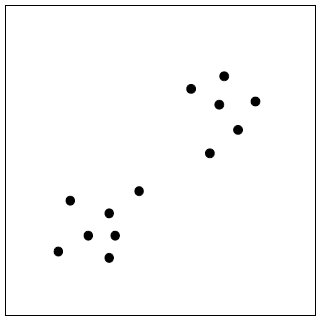
\includegraphics[width=1\linewidth,height=\textheight,keepaspectratio]{../../images/AA/kmeans1.jpg}
\end{center}
\end{block}
\end{frame}

\begin{frame}{Método k-médias (\emph{k-means})}
\phantomsection\label{muxe9todo-k-muxe9dias-k-means-2}
\begin{block}{Esquematicamente}
\phantomsection\label{esquematicamente-1}
\begin{center}
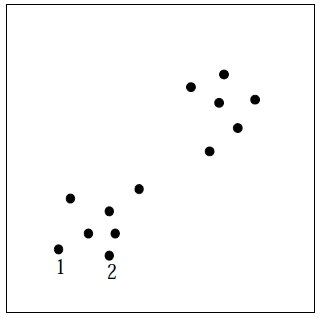
\includegraphics[width=1\linewidth,height=\textheight,keepaspectratio]{../../images/AA/kmeans2.jpg}
\end{center}
\end{block}
\end{frame}

\begin{frame}{Método k-médias (\emph{k-means})}
\phantomsection\label{muxe9todo-k-muxe9dias-k-means-3}
\begin{block}{Esquematicamente}
\phantomsection\label{esquematicamente-2}
\begin{center}
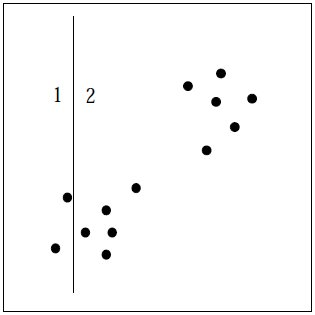
\includegraphics[width=1\linewidth,height=\textheight,keepaspectratio]{../../images/AA/kmeans3.jpg}
\end{center}
\end{block}
\end{frame}

\begin{frame}{Método k-médias (\emph{k-means})}
\phantomsection\label{muxe9todo-k-muxe9dias-k-means-4}
\begin{block}{Esquematicamente}
\phantomsection\label{esquematicamente-3}
\begin{center}
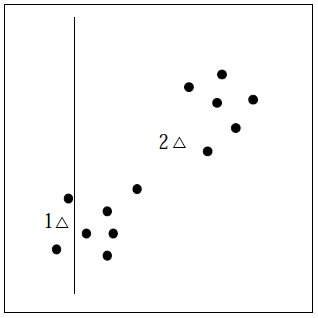
\includegraphics[width=1\linewidth,height=\textheight,keepaspectratio]{../../images/AA/kmeans4.jpg}
\end{center}
\end{block}
\end{frame}

\begin{frame}{Método k-médias (\emph{k-means})}
\phantomsection\label{muxe9todo-k-muxe9dias-k-means-5}
\begin{block}{Esquematicamente}
\phantomsection\label{esquematicamente-4}
\begin{center}
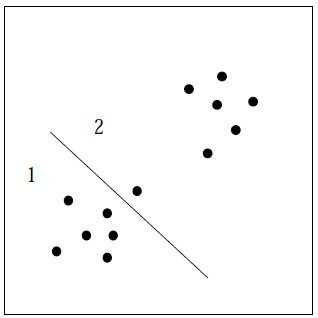
\includegraphics[width=1\linewidth,height=\textheight,keepaspectratio]{../../images/AA/kmeans5.jpg}
\end{center}
\end{block}
\end{frame}

\begin{frame}{Método k-médias (\emph{k-means})}
\phantomsection\label{muxe9todo-k-muxe9dias-k-means-6}
\begin{block}{Esquematicamente}
\phantomsection\label{esquematicamente-5}
\begin{center}
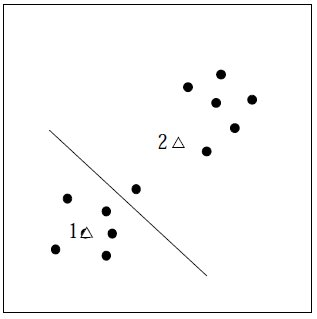
\includegraphics[width=1\linewidth,height=\textheight,keepaspectratio]{../../images/AA/kmeans6.jpg}
\end{center}
\end{block}
\end{frame}

\begin{frame}{Método k-médias (\emph{k-means})}
\phantomsection\label{muxe9todo-k-muxe9dias-k-means-7}
\begin{block}{Esquematicamente}
\phantomsection\label{esquematicamente-6}
\begin{center}
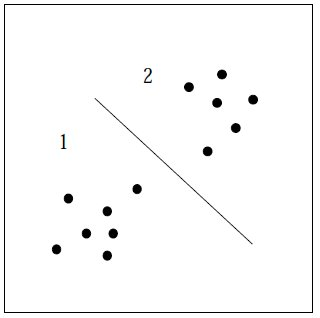
\includegraphics[width=1\linewidth,height=\textheight,keepaspectratio]{../../images/AA/kmeans7.jpg}
\end{center}
\end{block}
\end{frame}

\begin{frame}{Método k-médias (\emph{k-means})}
\phantomsection\label{muxe9todo-k-muxe9dias-k-means-8}
\begin{block}{Esquematicamente}
\phantomsection\label{esquematicamente-7}
\begin{center}
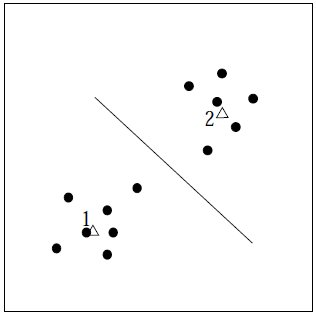
\includegraphics[width=1\linewidth,height=\textheight,keepaspectratio]{../../images/AA/kmeans8.jpg}
\end{center}
\end{block}
\end{frame}

\begin{frame}{Método k-médias (\emph{k-means})}
\phantomsection\label{muxe9todo-k-muxe9dias-k-means-9}
\begin{block}{Esquematicamente}
\phantomsection\label{esquematicamente-8}
\begin{center}
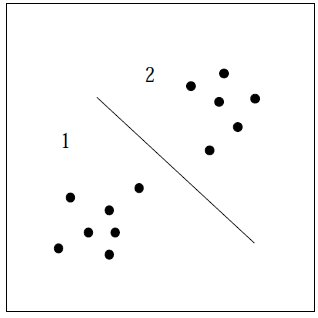
\includegraphics[width=1\linewidth,height=\textheight,keepaspectratio]{../../images/AA/kmeans9.jpg}
\end{center}
\end{block}
\end{frame}

\begin{frame}{Método k-médias (\emph{k-means})}
\phantomsection\label{muxe9todo-k-muxe9dias-k-means-10}
\begin{block}{Esquematicamente}
\phantomsection\label{esquematicamente-9}
\begin{center}
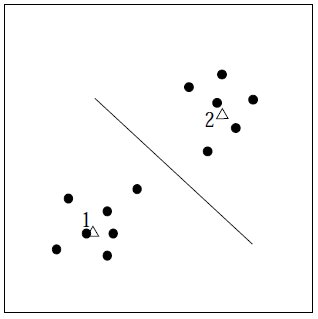
\includegraphics[width=1\linewidth,height=\textheight,keepaspectratio]{../../images/AA/kmeans10.jpg}
\end{center}
\end{block}
\end{frame}

\begin{frame}{Método k-médias (\emph{k-means})}
\phantomsection\label{muxe9todo-k-muxe9dias-k-means-11}
\begin{block}{Esquematicamente}
\phantomsection\label{esquematicamente-10}
\begin{center}
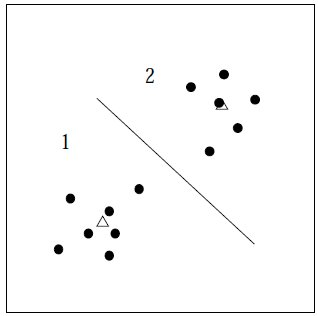
\includegraphics[width=1\linewidth,height=\textheight,keepaspectratio]{../../images/AA/kmeans11.jpg}
\end{center}
\end{block}
\end{frame}

\begin{frame}{Método k-médias: comentários finais}
\phantomsection\label{muxe9todo-k-muxe9dias-comentuxe1rios-finais}
\begin{itemize}
\tightlist
\item
  O algoritmo \textit{k-means} é sensível à configuração inicial dos
  clusters (passo \(a)\)), podendo produzir resultados diferentes
  mediante diferentes partições iniciais.
\end{itemize}

\pause

\begin{itemize}
\tightlist
\item
  O usual é considerar, inicialmente, \(k\) ``sementes'', que seriam
  \(k\) pontos definidos em \(R^p\).
\end{itemize}

\pause

\begin{itemize}
\tightlist
\item
  O processo inicia alocando cada elemento à semente mais próxima, e
  atualizando o ponto de referência do cluster (centroide) cada vez que
  ele incorpora um novo elemento.
\end{itemize}

\pause

\begin{itemize}
\tightlist
\item
  Podemos definir as sementes como os vetores de observações de \(k\)
  elementos selecionados aleatoriamente da base.
\end{itemize}
\end{frame}

\begin{frame}{Método k-médias: comentários finais}
\phantomsection\label{muxe9todo-k-muxe9dias-comentuxe1rios-finais-1}
\begin{itemize}
\tightlist
\item
  \textbf{Nota:} Estabelecer alguma restrição quanto à distância das
  sementes, garantindo alguma distância mínima entre elas, pode ajudar
  na performance do método.
\end{itemize}

\pause

\begin{itemize}
\tightlist
\item
  As sementes podem ser definidas como \(k\) vetores quaisquer definidos
  em \(R^p\);
\end{itemize}

\pause

\begin{itemize}
\tightlist
\item
  Caso se considere algum mecanismo aleatório de seleção de sementes, é
  recomendável que o processo seja repetido um número \(m\) de vezes,
  identificando-se, dentre as \(m\) soluções obtidas, a solução ótima;
\end{itemize}
\end{frame}

\begin{frame}{Método k-médias: comentários finais}
\phantomsection\label{muxe9todo-k-muxe9dias-comentuxe1rios-finais-2}
\begin{itemize}
\tightlist
\item
  Uma alternativa é rodar, inicialmente, uma análise hierárquica, e
  definir \(k\) clusters;
\end{itemize}

\pause

\begin{itemize}
\tightlist
\item
  Os centroides dos \(k\) clusters obtidos podem servir de semente para
  o algoritmo \emph{k - means}.
\end{itemize}
\end{frame}




\end{document}
